\documentclass[10pt,a4paper]{article}
\usepackage[utf8]{inputenc}

\usepackage{amsmath}
\usepackage{amsfonts}
\usepackage{amssymb}
\usepackage{graphicx}
\usepackage{listings}
\usepackage[margin=1.0in]{geometry}
\usepackage{caption}
\usepackage{subcaption}
\usepackage{float}
\usepackage[utf8]{inputenc}
\usepackage{refstyle}
\usepackage{wrapfig}
\usepackage{comment}
\usepackage{wrapfig}
\usepackage{hyperref}


\lstset{numbers=left,
	title=\lstname,
	numberstyle=\tiny,
	breaklines=true,
	tabsize=4,
	language=Python,
	morekeywords={with,super,as},,
	frame=single,
	basicstyle=\footnotesize\tt,
	commentstyle=\color{comment},
	keywordstyle=\color{keyword},
	stringstyle=\color{string},
	backgroundcolor=\color{background},
	showstringspaces=false,
	numbers=left,
	numbersep=5pt,
	literate=
		{�}{{\ae}}1
		{�}{{\aa}}1
		{�}{{\o}}1
		{�}{{\AE}}1
		{�}{{\AA}}1
		{�}{{\O}}1
	}
\usepackage{setspace}
\doublespacing
\usepackage{bm}
\usepackage{hyperref}

\begin{document}

\begin{center}
{\LARGE\bf ProMax Exercise\\GEO4280}
\\


\includegraphics[scale=0.1]{UiO.jpg}\\


Authors: Robin David Kifle, Julie Linnea Gresseth, Sander Losnedahl
\\
{\large\bf Abstract}
\end{center}

\noindent Seismic data is used to get an understanding of the subsurface, but many processes must be applied to the raw data for the image to be a sufficiently accurate depiction of the subsurface. This paper presents a workflow where different processing techniques like muting, amplitude recovery, bandpass filtering, deconvolution, NMO-correction, stacking and migration are applied to a raw data set in the ProMax software. It will show the importance of signal processing and how it helps us get a better image of the subsurface. The paper has found that a combination of the above techniques yields good results and removes effects like direct wave and top refractors, unwanted frequencies, multiples, normal move-out, dipping reflectors and diffraction hyperbolas. The two different migrations used (finite-difference and Kirchhoff) gave similar results, except for data related to salt and muting.

\newpage

\tableofcontents

\newpage

\section{Introduction}

Seismic processing consists of employing algorithms to recorded data in order to obtain an image that represent the subsurface and facilitates seismic interpretation. The received seismic response is a mixture of the source pulse, the Earths response and background noise. In this project we will learn to use the ProMAX Software for processing one 2D line. The main goal of the project is to get to know the workflow needed to get good results in terms of seismic imaging.


\section{Preprocessing and CMP-sorting}

\begin{figure}[H]
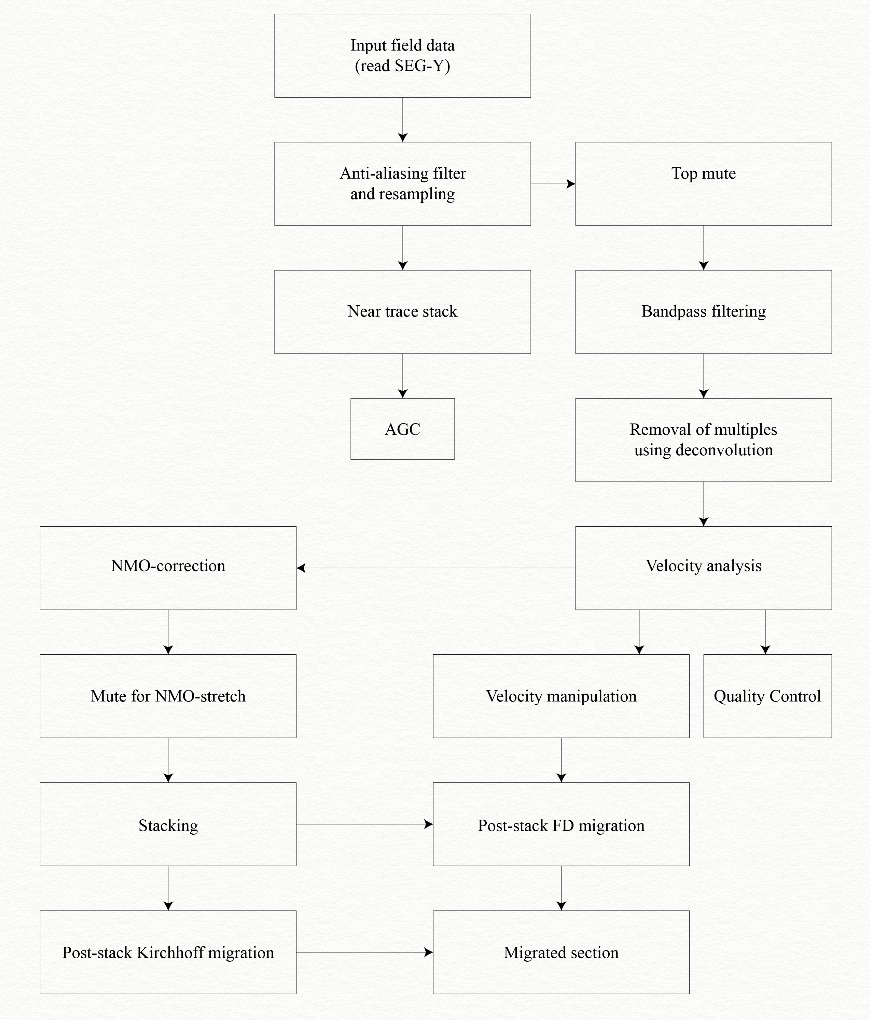
\includegraphics[scale=0.4]{wf3.jpg}
\caption{Entire workflow.}
\label{wf}
\end{figure}

With aim to generate a dataset better suited for further processing, preprocessing entails editing inadequate measurements, applying datuming and introducing wavelet corrections.\\
Usually the data have also gone through an anti-aliasing filter, and carefully resampled to reduce the amount of data. A broad bandpass filter removing very low ($<2Hz$) frequencies and very high frequencies might also have been used.
\\
Figure \ref{wf} illustrates någe
\\
The seismic data have been acquired in the source-receiver domain. The data needs to be resorted into CMP (common midpoint) gathers. Promax uses the abbreviation CDP (common depth point), even though CDP and CMP are only equivalent for horizontally layered reflectors.
\\
\noindent Seismic data acquisition is performed with a source and a receiver, giving a dataset consisting of several traces with various offsets and midpoints. CMP sorting is performed to resort the dataset in a midpoint-offset-domain, see figure \ref{fig1} for illustration. Traces with a common midpoint between sources and receivers are orderly gathered in CMP-gathers (Gelius, 2018a).

\begin{figure}[H]
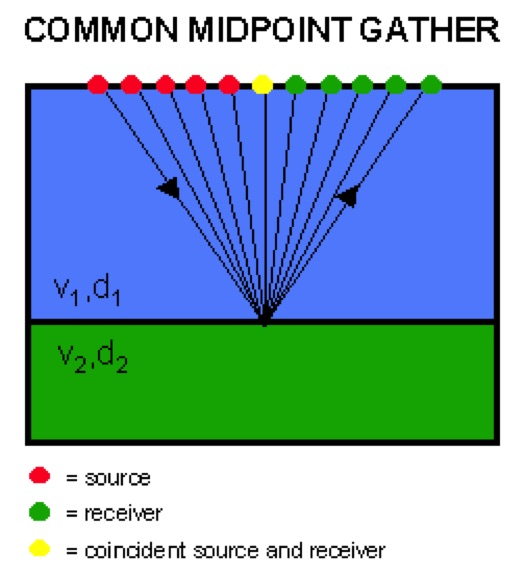
\includegraphics[scale=0.6]{fig1.jpg}
\caption{Illustrative figure showing the principle of CMP- sorting (XSGEO, 2015).}
\label{fig1}
\end{figure}

\subsection{Raw Data}

Raw seismic data containing traces of both direct, reflected and refracted waves, was converted from SEG-Y format to an internal processing format applicable in ProMAX. Maximum traces per ensemble was set to 240, and domain set to midpoint-offset. The output raw seismic data of CMP 1000 and CMP 1500 is shown in figure \ref{fig2}.

\begin{figure}[H]
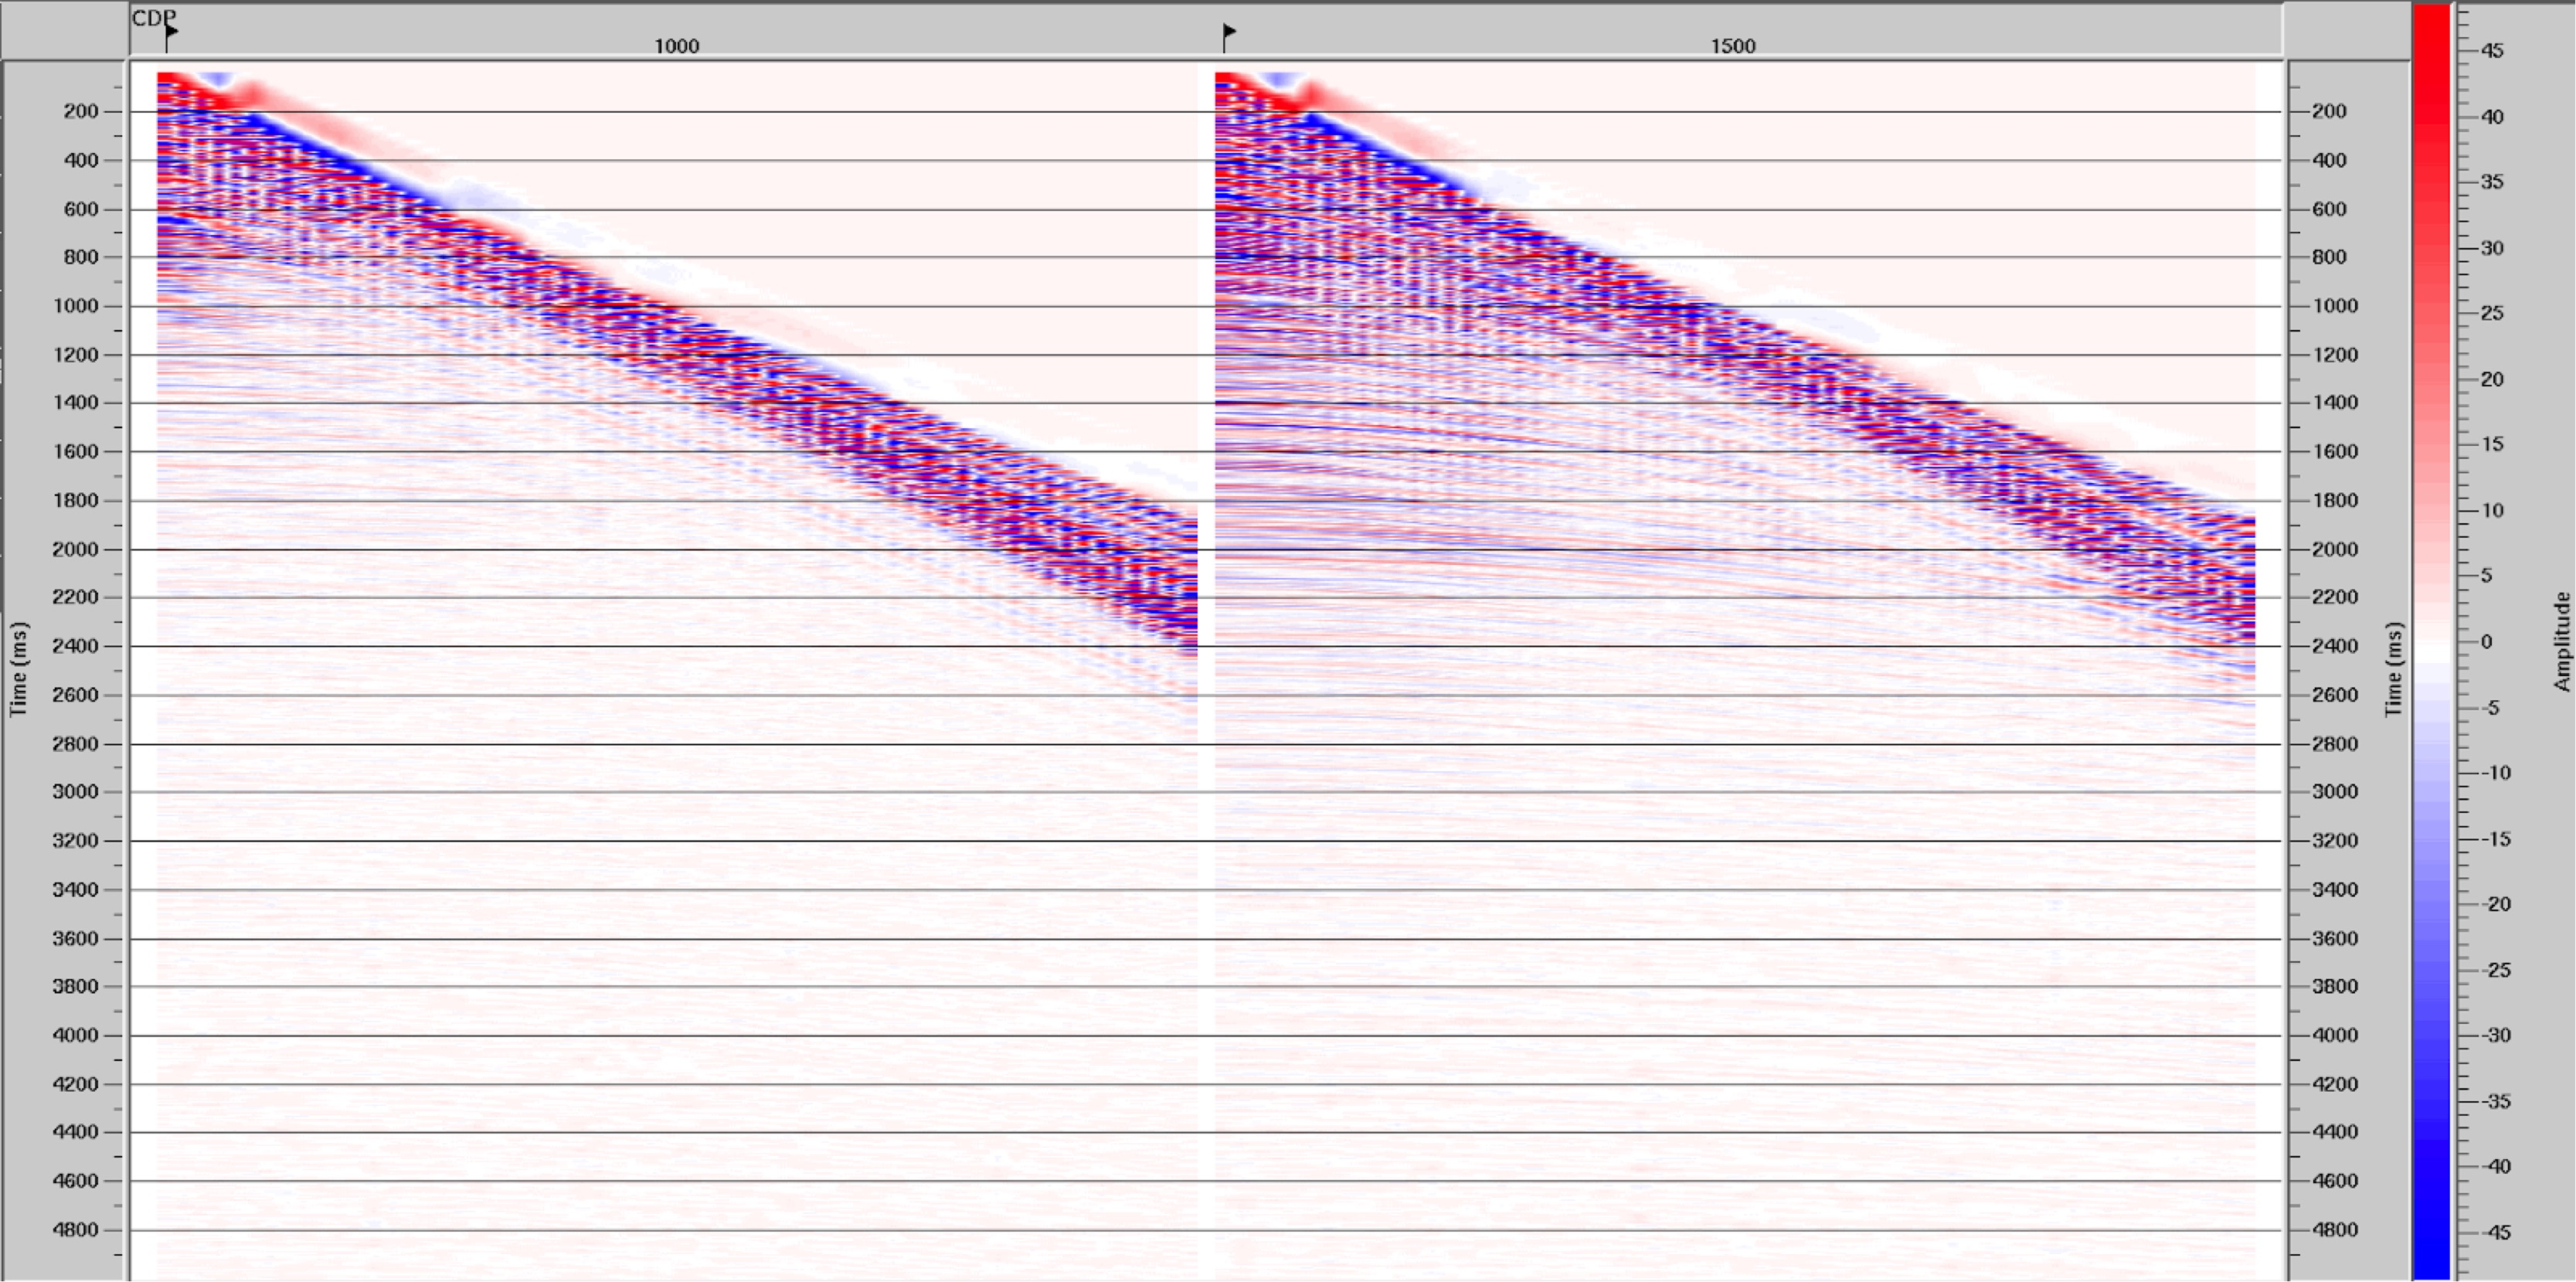
\includegraphics[width=\textwidth]{fig2.jpg}
\caption{Raw data of CMP 1000 (left) and 1500 (right).}
\label{fig2}
\end{figure}

\section{Near Trace Stack}


\subsection{Common Midpoint (CMP/Ensamble) Stack}

A stack may be defined as a processed seismic record that consists of a series of traces that have been added together. Stacking is performed to improve the signal-to-noise (S/N) -ratio and improve overall data quality. The number of traces added together is referred to as the fold, where a higher fold provides enhanced resolution (Gillis, 2018a; Gelius, 2018a).
\\
A CMP stack is hence generated by adding together CMP-data at different offsets and a common reflection point, to form a single trace. A near-trace stack was made using only the traces closest to the air gun array (108-133 meters), without further processing of the data, see figure \ref{fig3}. The following observations were made:

\begin{itemize}
    \item strong amplitudes in the shallow part, increasing amplitude loss with depth
    \item the outline of a domal structure is observed also in the shallow part, but vertical extent is somewhat ambiguous due to lack of amplitude in depth
\end{itemize}

\subsection{Amplitude Recovery}

Amplitude recovery aims to correct for amplitude loss, which may be caused by three major factors:

\begin{itemize}
    \item geometrical spreading: progressive decay of wave energy caused by increasing wavefront area as the wave propagates ($t^2$)
    \item intrinsic attenuation/anelasticity: energy loss due to internal friction which causes conversion of some of the seismic elastic energy to heat
    \item transmission losses: loss of wave amplitude due to reflection at interfaces (Gelius, 2018a)
\end{itemize}

\noindent To correct for amplitude attenuation several approaches may be employed. These are generally divided into two categories:
\\
\\
{\bf Deterministic approach}
\\
The t-square model is one amongst several deterministic approaches, using the fact that geometrical spreading scales the wave amplitude as $\frac{1}{r}$ and the wave energy as $\frac{1}{r^2}$, where r is distance from the source. Assuming a constant velocity, the travel time, t, is then proportional to the distance, r, a correction factor of $t^a$, where a is an integer and t is the travel time, may be used. This results in an an amplitude adjustment in the form of scaling the deeper parts of the data more than in the upper part.
\\
\\
{\bf Statistical Approach}
\\
One type of statistical amplitude recovery commonly used is the Automatic Gain Control (AGC), applied to account for energy loss at higher TWT. This is referred to as scaling since the traces at higher TWT and lower TWT are disproportionately scaled to regain reflector energy and obtain visibility (Gelius, 2018a; Gillis, 2018b). AGC was used in this workflow for this exact purpose, see figure \ref{fig4}.


\begin{figure}[H]
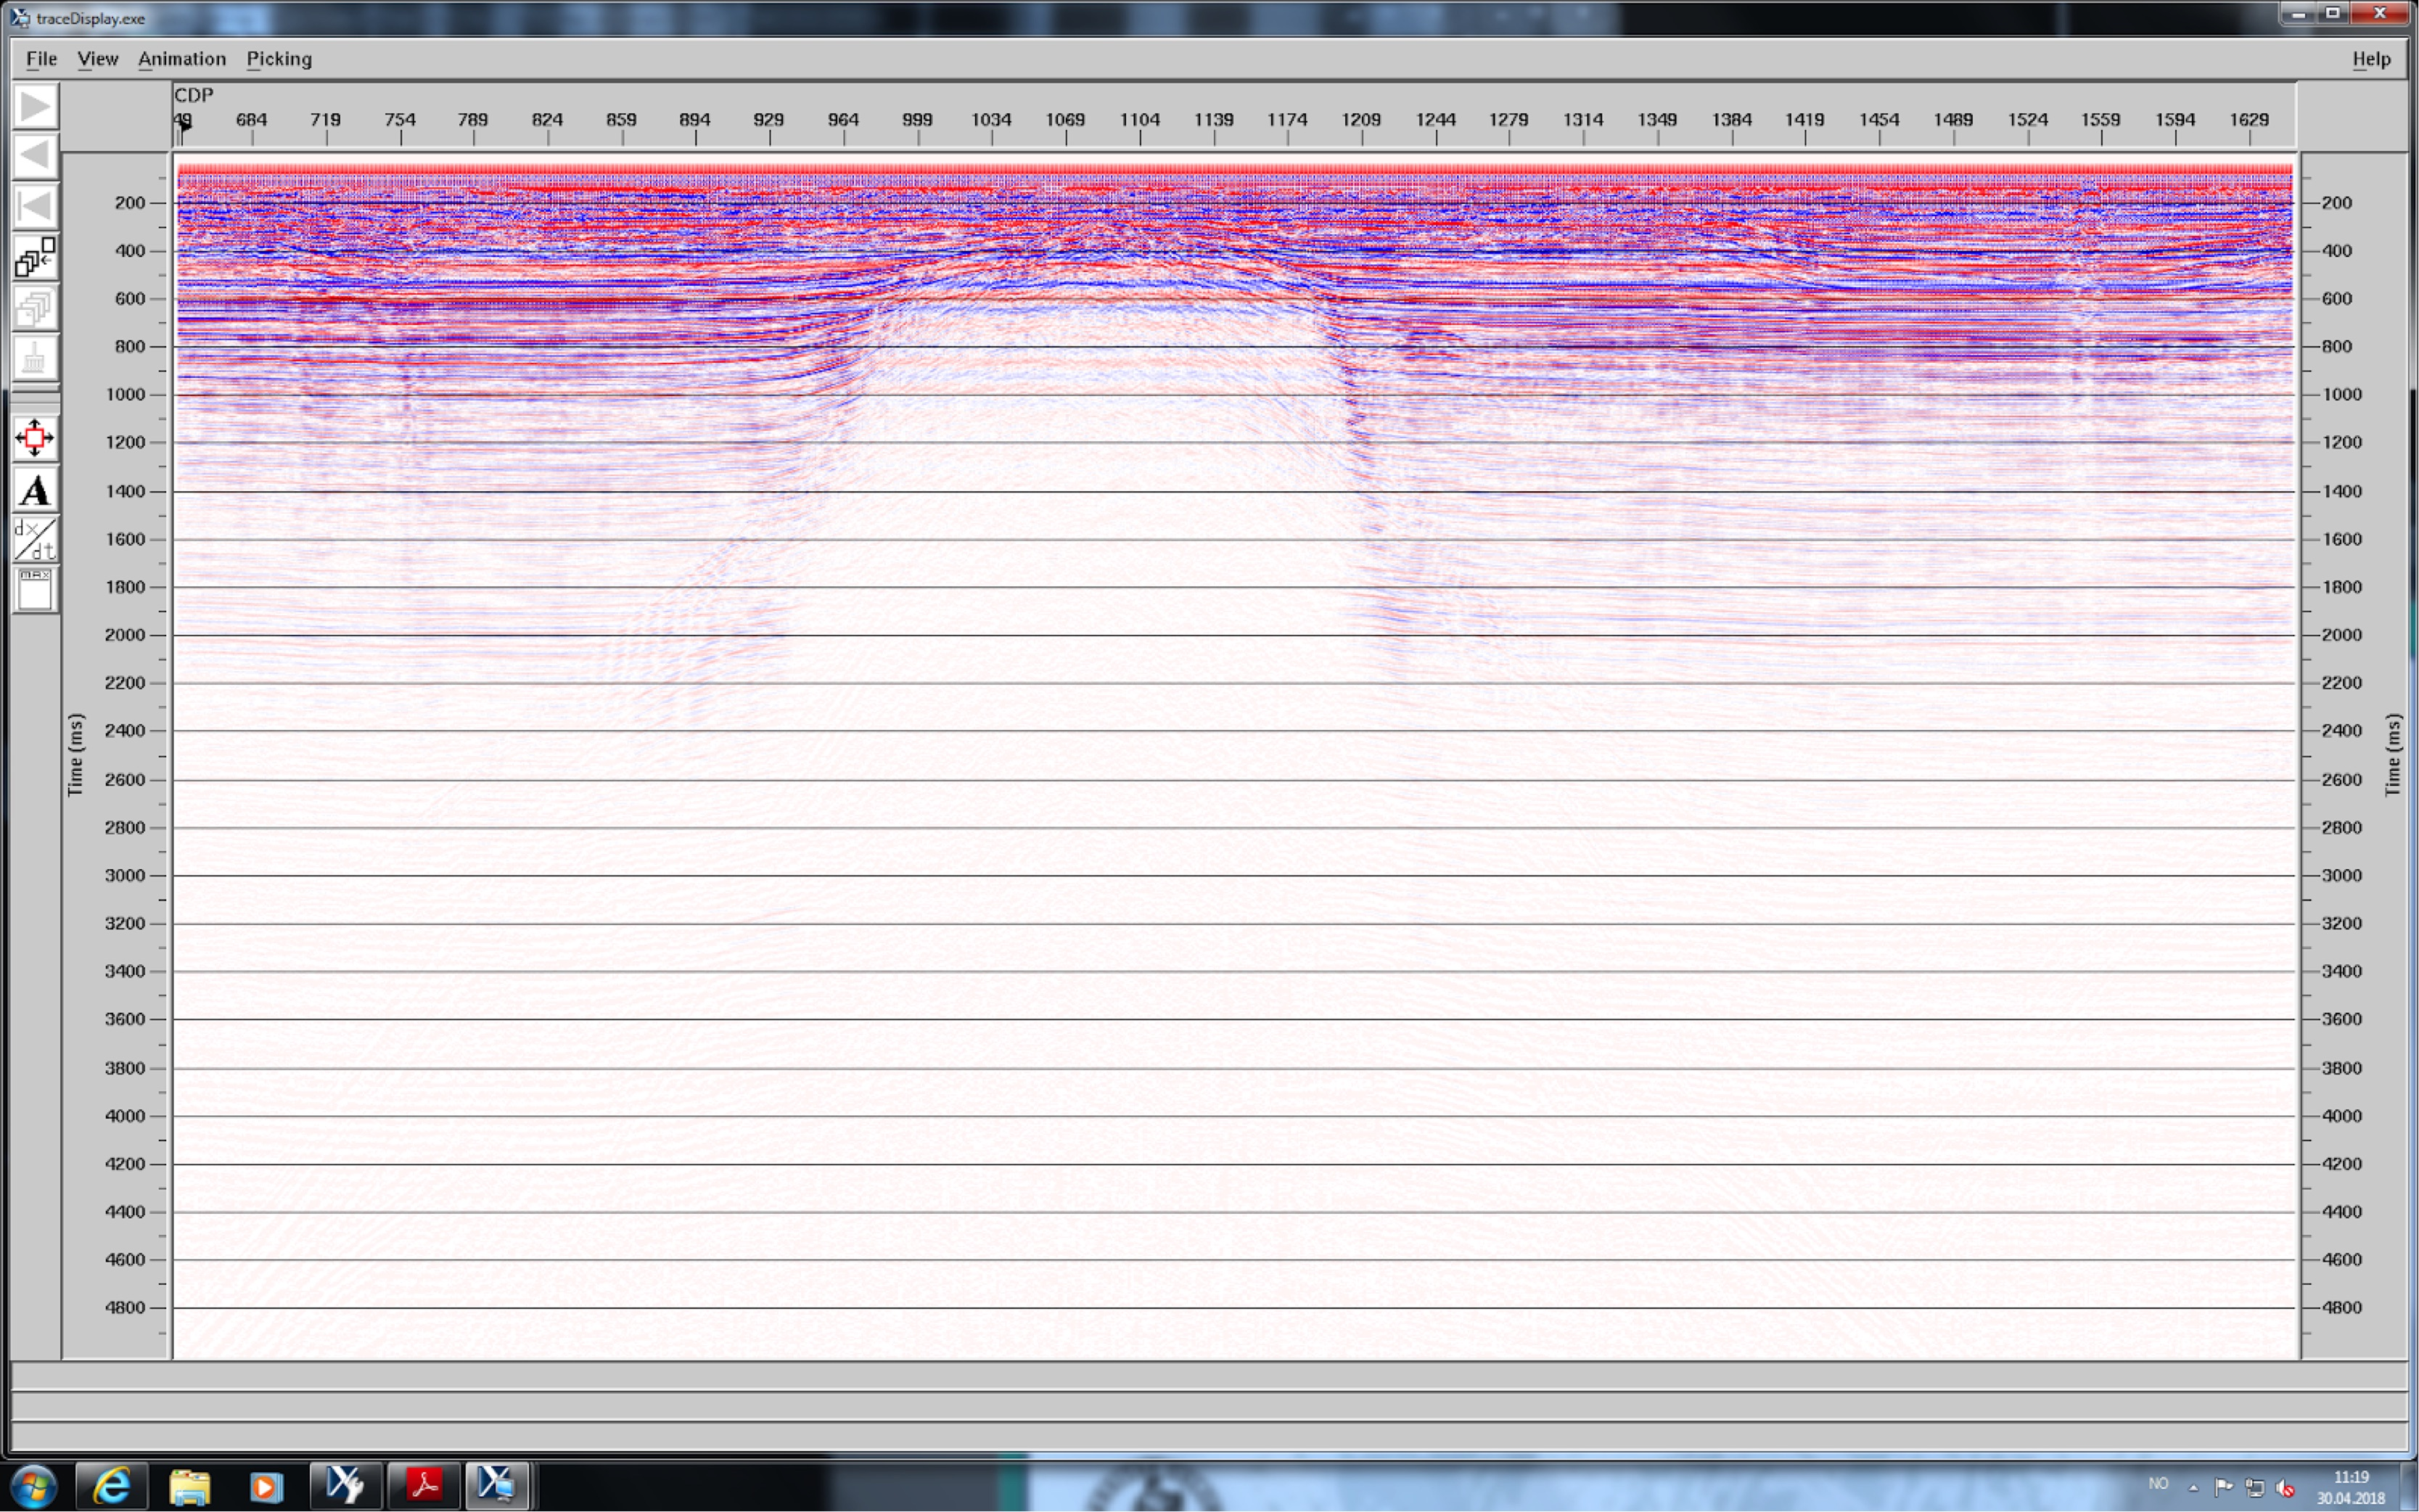
\includegraphics[width=\textwidth, trim={1.5cm 1.5cm 1cm 1.5cm},clip]{fig3.jpg}
\caption{Near-trace stack prior to scaling. Strong amplitudes are solemnly found in the shallowest regions and appear progressively weaker with increasing depth. The contours of a dome structure is visible in the centre of image, but vertical extent is hard to determine due to lacking imaging in the deeper sections.}
\label{fig3}
\end{figure}

\begin{figure}[H]
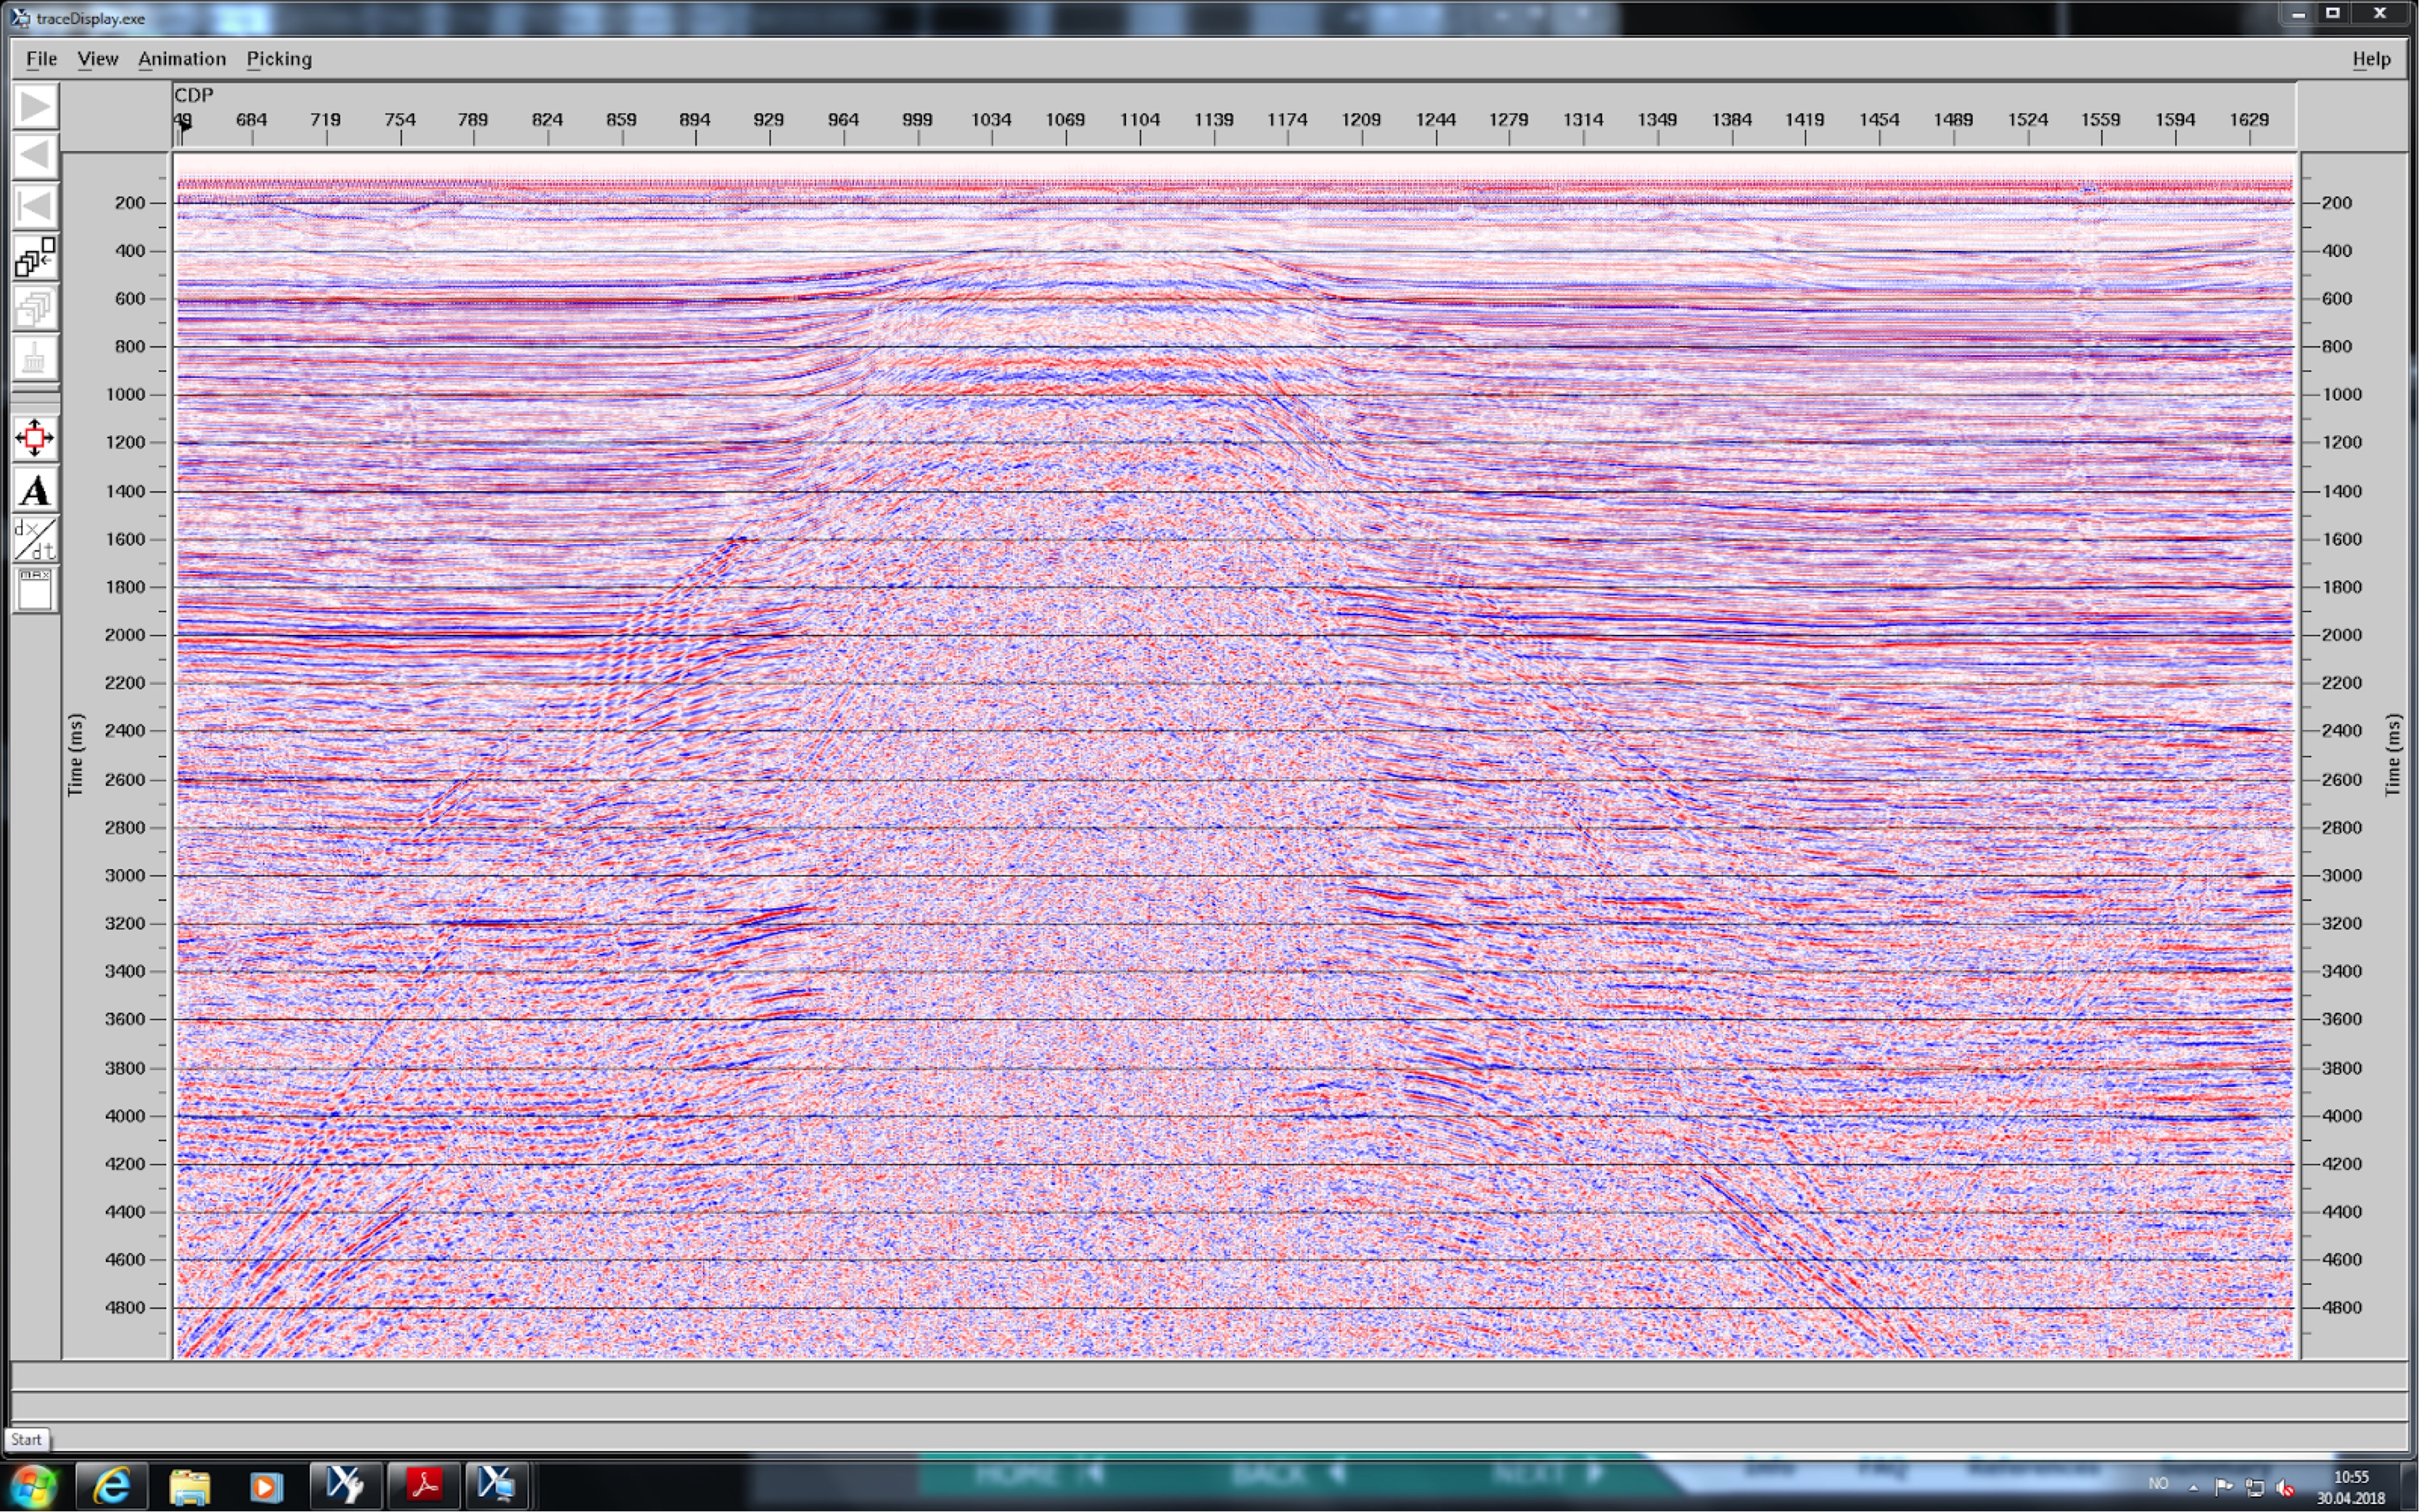
\includegraphics[width=\textwidth, trim={1.5cm 1.5cm 1cm 1.5cm},clip]{fig4.jpg}
\caption{Near-trace-stack after scaling, showing recovered amplitudes in the deeper part. Strong reflectors are revealed in the deeper parts, defining the contours of the dome structure, thus generating a better image of the subsurface.}
\label{fig4}
\end{figure}


\noindent By comparing figure \ref{fig3} and \ref{fig4}, the effect of amplitude recovery is highly detectable. In figure \ref{fig4} amplitudes are amplified at larger travel times, and thus shows displays increasing visibility of later arriving events, not previously visible (figure \ref{fig5}). The recovered reflectors shows varying amplitudes through seemingly sedimentary layers. The outline of the domal structure is visible in the deeper sections, showing what at first glance resembles a salt dome with great vertical extent.

\section{Data Processing}

\subsection{Muting and Scaling}

Muting removes data above (or below) a certain time gradient, aiming to improve data quality by noise in dataset. Muting may also be utilized to remove the effect of NMO-stretching (Gelius, 2018a). 
\\
A mute function was applied to the raw dataset, removing the effects of the direct and refracted waves prior to deconvolution. A time gradient was given as input and a top mute was applied, removing all the lower time values. Applying a too strong or too mild time gradient preserves too much or too little of the traces at low travel times in the CMP-gather, respectively. A proper choice of mute function leads to only a few, but clear traces at low travel times, see figure \ref{fig5} for examples. Removing he direct wave and top refractors improves the S/N ratio.


\begin{figure}[H]
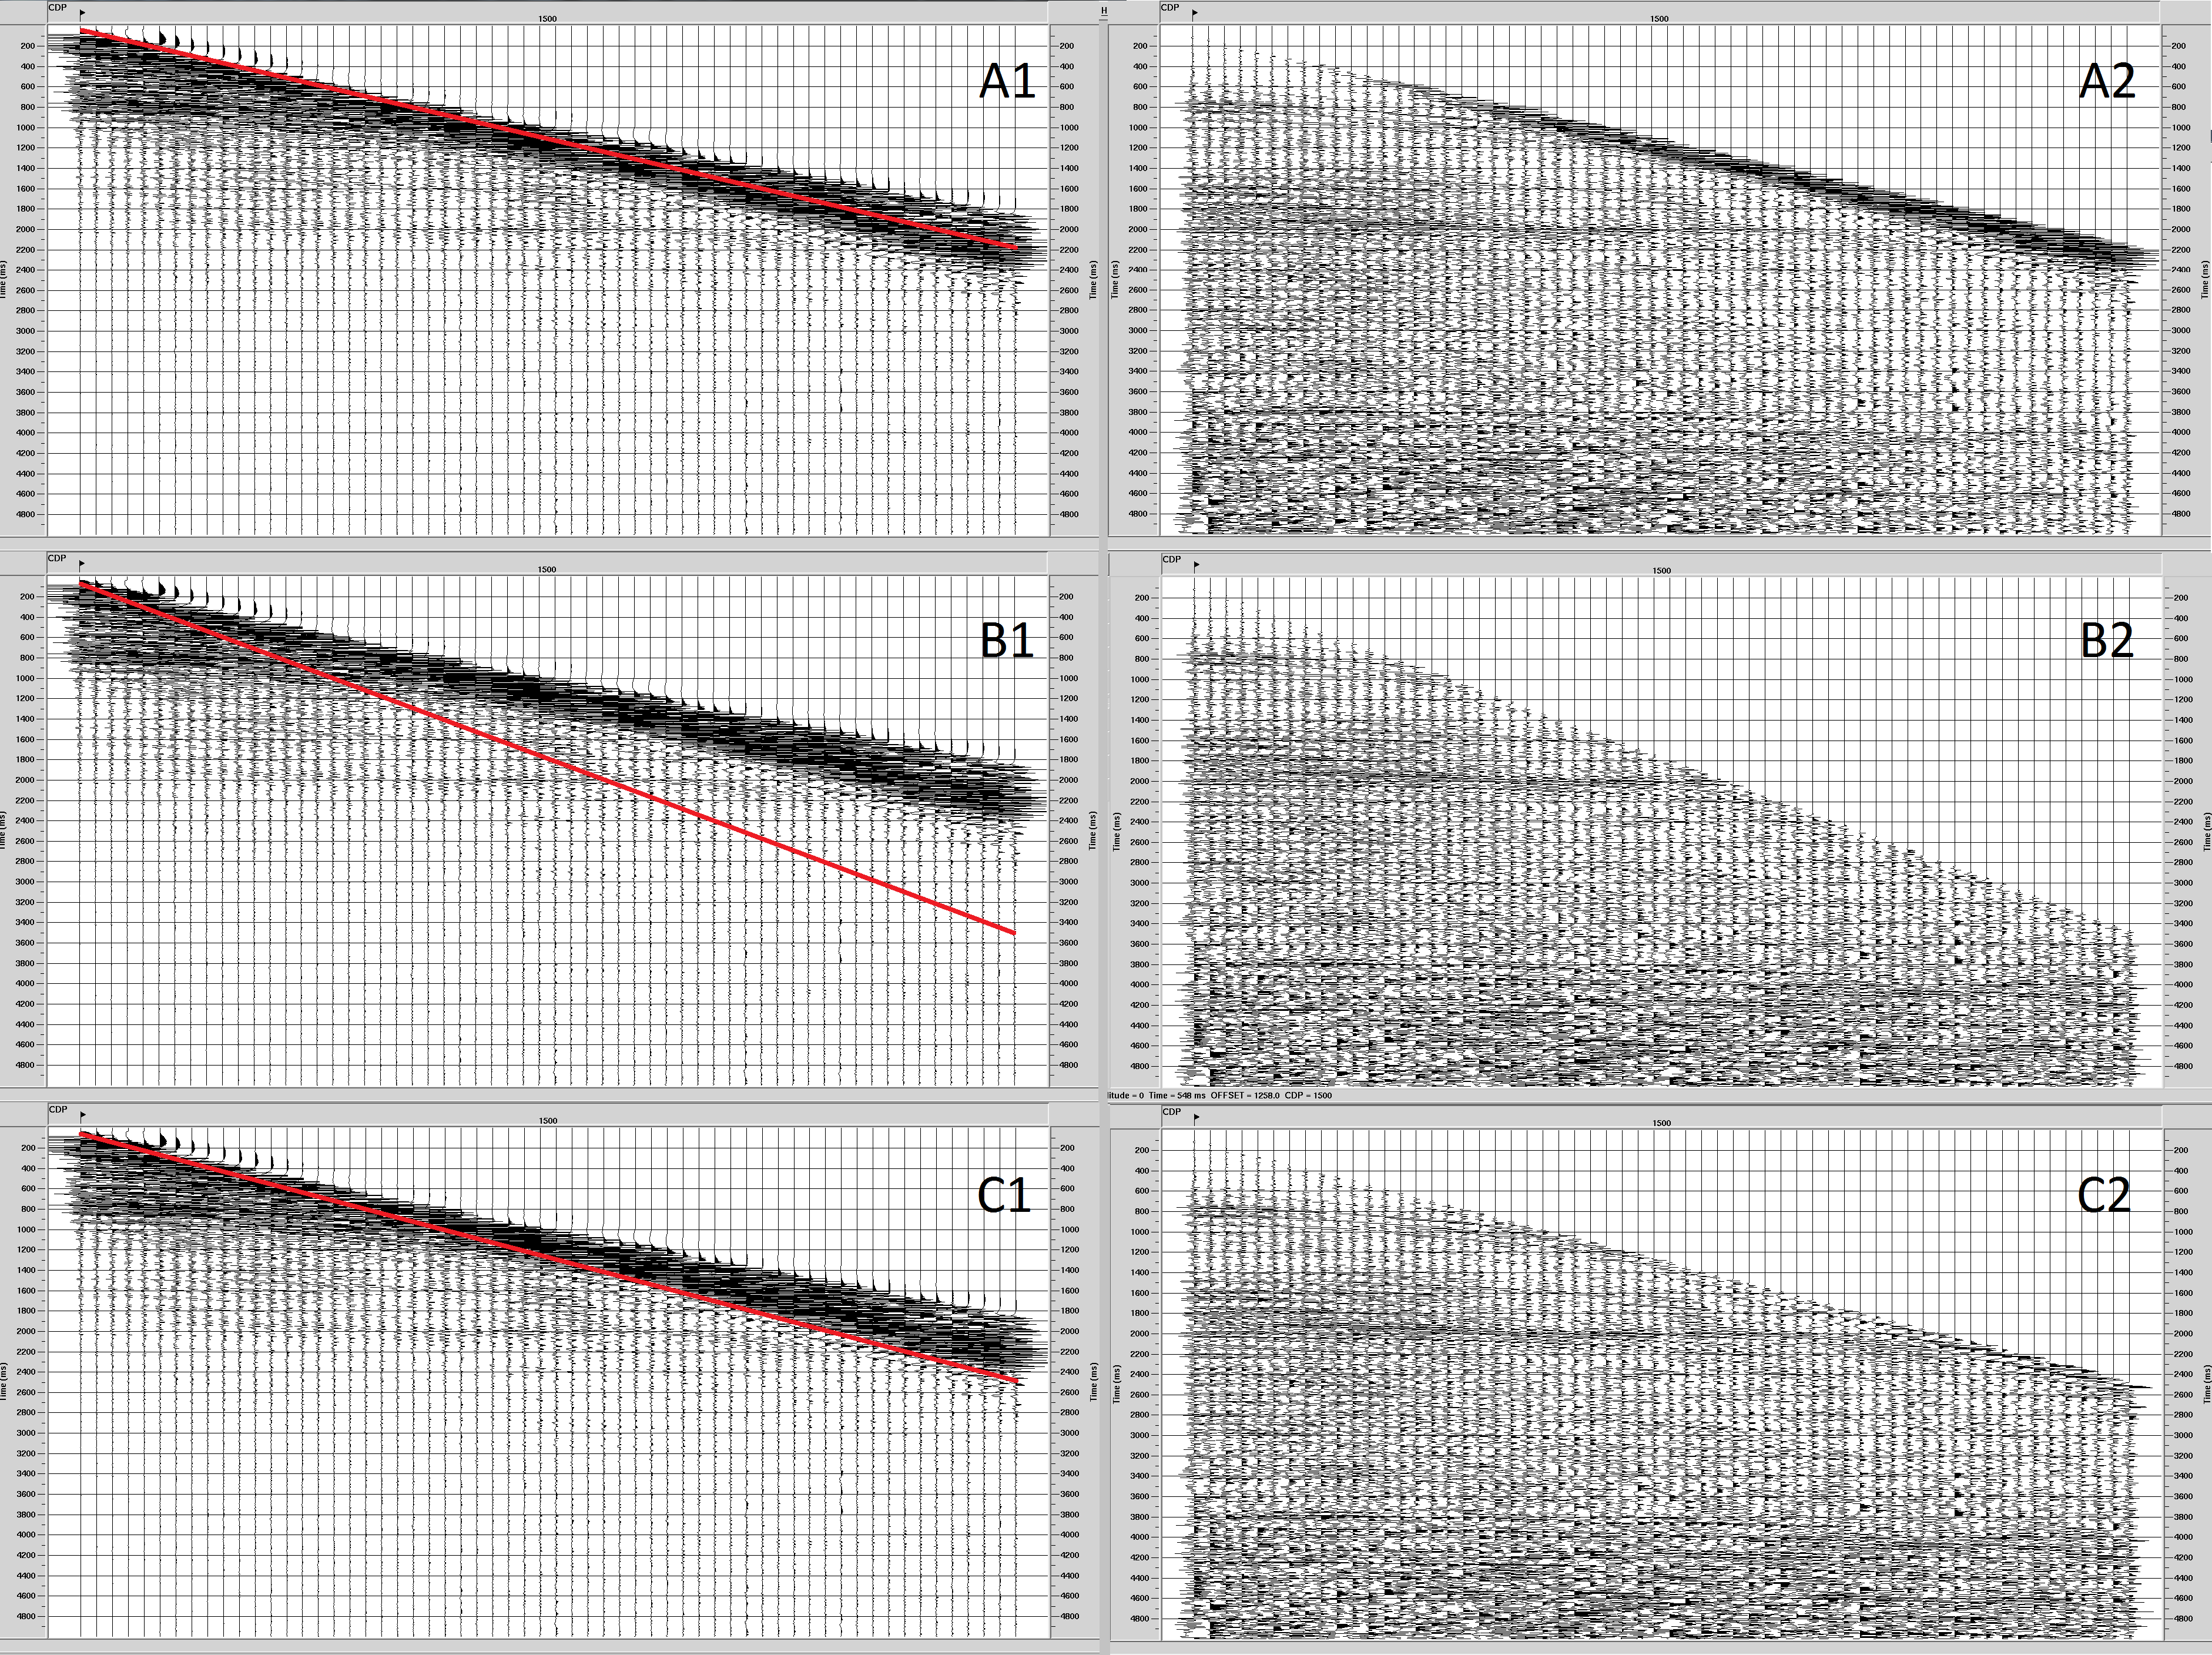
\includegraphics[width=\textwidth]{fig5.jpg}
\caption{Comparison of CMP 1500 before, denoted 1, and after, denoted 2, muting and scaling. The mute line is marked in black on the raw data in A1-C1. A2-C2 shows muted and amplitude recovered data by employing $t^3$. A2 and B2 shows the effect of employing a too strong or too mild mute function, respectively. C2 shows the result of correct muting.}
\label{fig5}
\end{figure}


\noindent To address challenges related to amplitude attenuation/energy loss (discussed in chapter 2.2), amplitude recovery through scaling was performed on the data. True Amplitude Recovery, a ProMax-function based on the t-square model, was used to recover amplitudes in the deeper section (ProMax, 2018). The integer factor a was set to 3. The results of muting and scaling for CMP 1000 and CMP 1500 can be seen in figure \ref{fig6}.  

\begin{figure}[H]
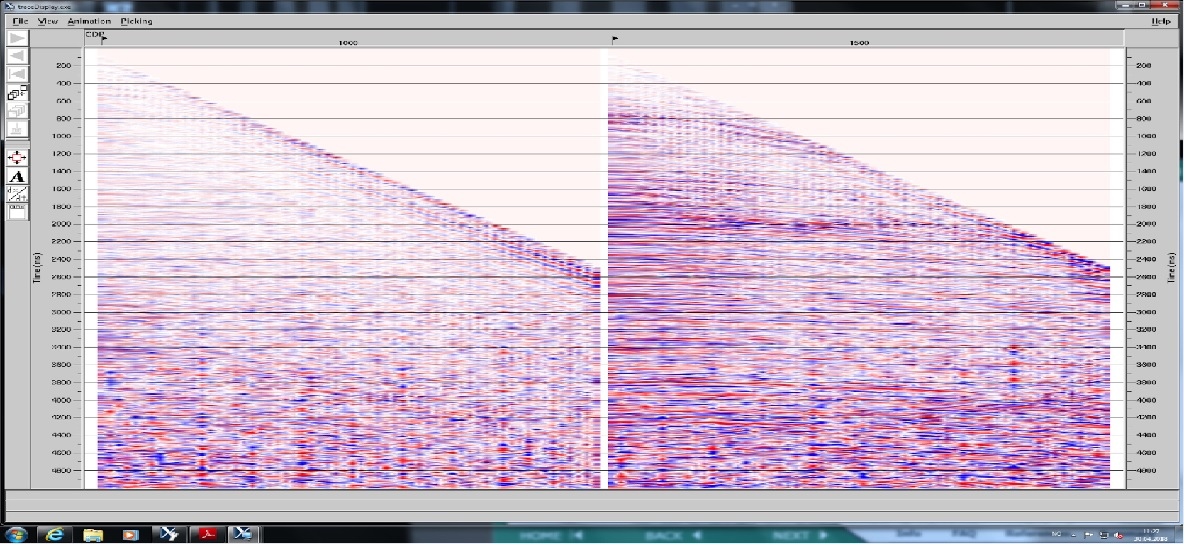
\includegraphics[width=\textwidth, trim={1.5cm 1.5cm 1cm 1.5cm},clip]{fig6.jpg}
\caption{CMP 1000 (right) and 1500 (left) after both scaling and muting.}
\label{fig6}
\end{figure}

\noindent To more accurately compare data, wiggle-trace and plot equalization are used. The wiggle trace displays variations in each trace relative to the x-axis corresponding to its receiver location. Positive deviations, peaks, are seen shaded on the left and negative deviations, throughs, are seen unshaded on the right of the wiggle-trace centre. The purpose of this display is to also show the weaker reflections and their correlative changes (Gelius, 2018a). 
\\
Figure \ref{fig7} and \ref{fig8} illustrates through zoomed sections the effects of muting and scaling for CMP 1500. While applying a mute function effectively removed direct and refracted rays, the scaling removed the effect of seismic attenuation by recovering amplitudes at larger traveltimes. 


\begin{figure}[H]
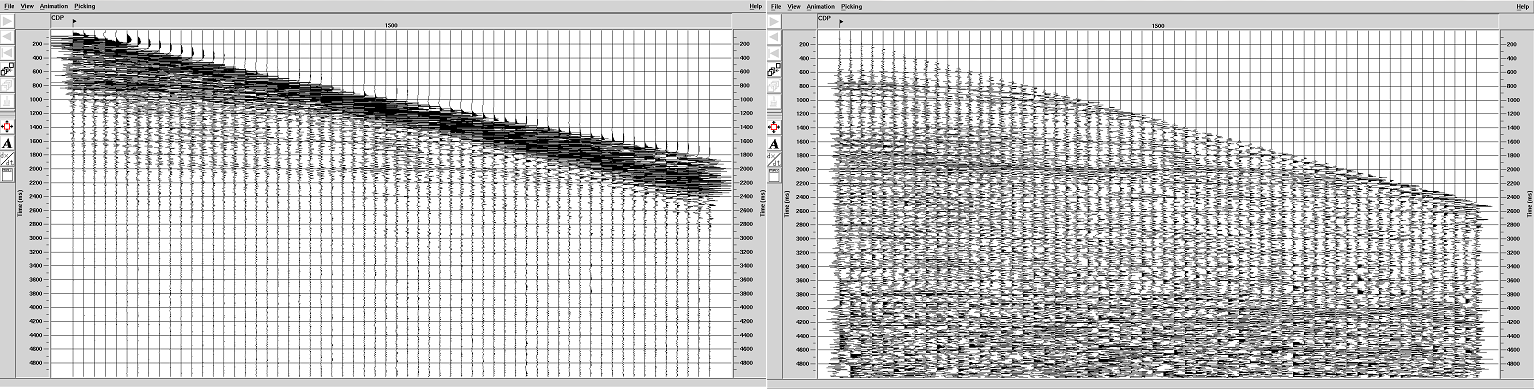
\includegraphics[width=\textwidth]{fig7ekte.jpg}
\caption{Comparing CMP 1500 before (left) and after (right) both muting and scaling, to better image the amplitudes which are recovered in the scaled data and the removal of data above mute line.}
\label{fig7}
\end{figure}



\begin{figure}[H]
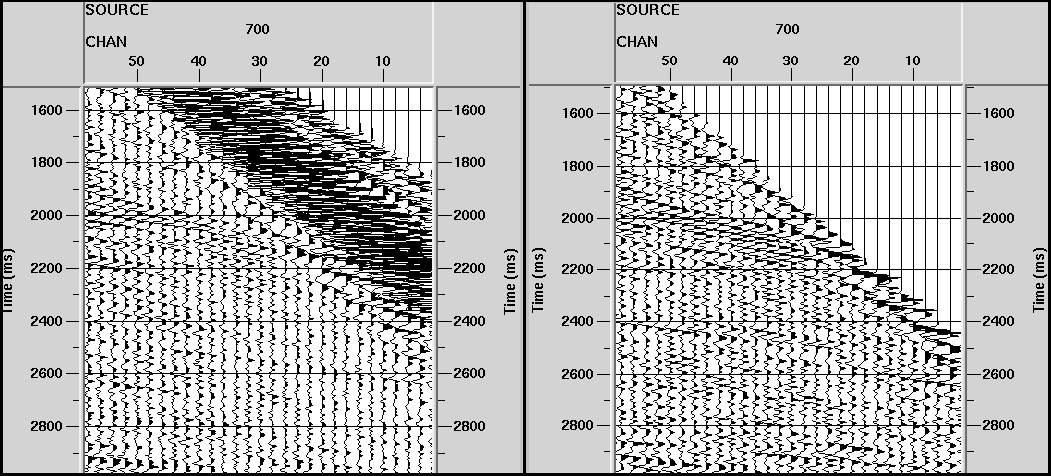
\includegraphics[width=\textwidth]{fig8.jpg}
\caption{Cut-out of times from 1500-3000 ms, comparing scaled CMP 1500 before (left) and after (right) muting. Notice that refracted and direct rays have been zeroed out due to muting. Amplitudes are also recovered at deeper travel-times, this due to scaling.}
\label{fig8}
\end{figure}

\subsection{Bandpass Filtering}


To enhance the wanted signal and remove noise, filters are applied to the seismic data. Bandpass filters effectively remove unwanted parts of the data through passing only frequencies within a specific range, rejecting excessive frequencies. The aim is to remove ambient noise, such as the high frequencies produced by weather conditions, vibrations from machinery, platforms and passing vessels. The most facile way of constructing a bandpass filter is by defining it as a difference between two low-pass filters (Gelius, 2018a). 
\\
Two commonly used bandpass filters are the Butterworth and Ormsby-filters (Gelius 2018a). The Butterworth filter is recognized as a box-shaped filter in the frequency domain. For this exercise however, the Ormsby filter [f1, f2, f3, f4] was applied, which is a filter of trapezoidal shape where the corner frequencies define the range of the bandpass. The corners are denoted f1: low-cut frequency, f2: low-pass frequency, f3: high-pass frequency and f4: high-cut frequency, see figure \ref{fig9}.

\begin{figure}[H]
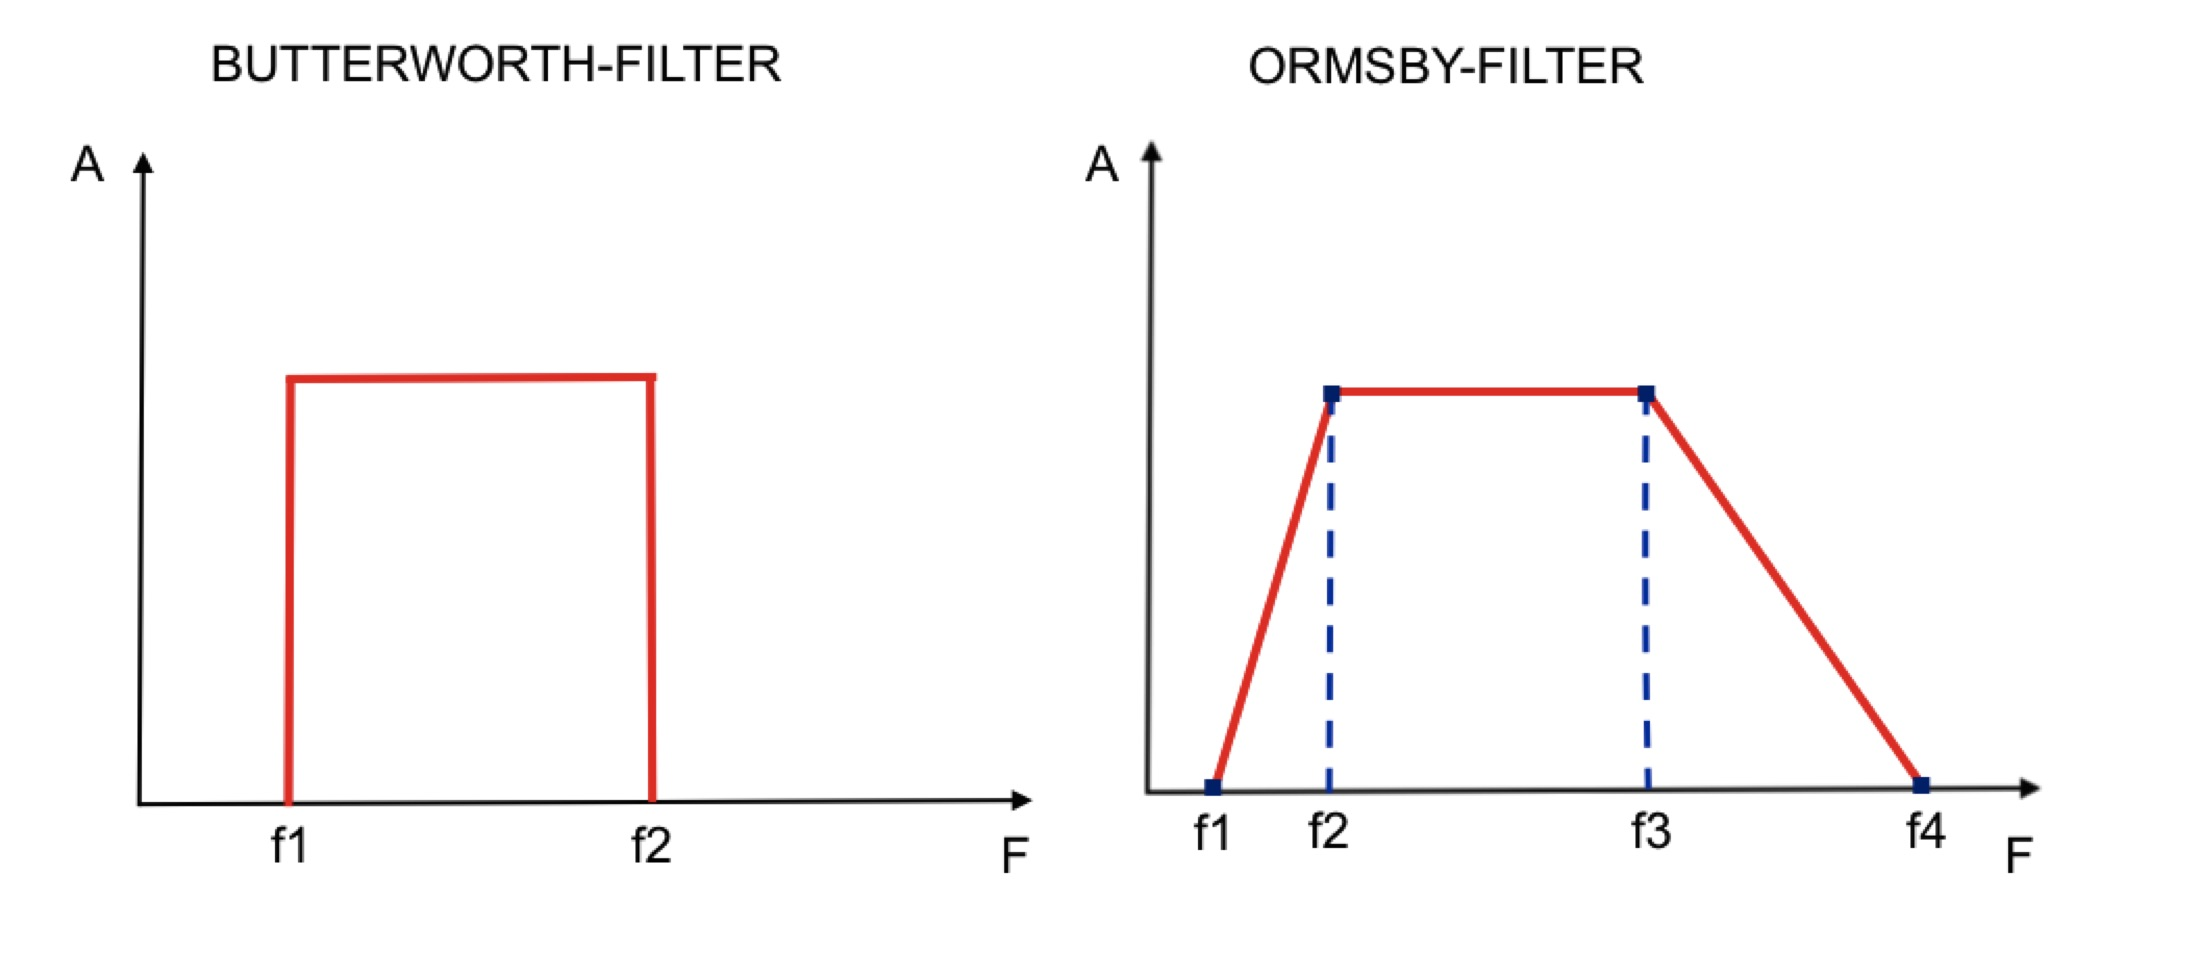
\includegraphics[width=\textwidth]{fig9.jpg}
\caption{Illustration of the characteristics of the boxshaped Butterworth (left) and trapezoidal Ormsby (right) -filters. A: amplitude, F: frequency.}
\label{fig9}
\end{figure}


\noindent If the slopes of the filter are too steep, the filter will act as a box-window and Gibb’s phenomenon may occur. The sinc-function may cause signal distortion in the form of oscillations corroding the amplitude spectrum, see figure \ref{fig10}. Optimally, such artifacts ought to be minimized by setting the f2-f3 interval significantly shorter than f1-f4, ensuring a trapezoidal rather than a box-shaped filter.

\begin{figure}[H]
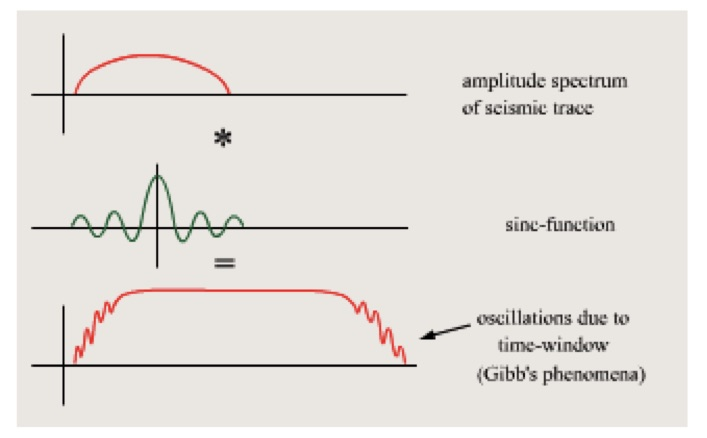
\includegraphics[width=\textwidth]{fig10.jpg}
\caption{Illustration of the signal distortion which may occur using a filter with too steep slopes, known as the Gibb’s phenomenon (Gelius, 2018a).}
\label{fig10}
\end{figure}


\begin{figure}[H]
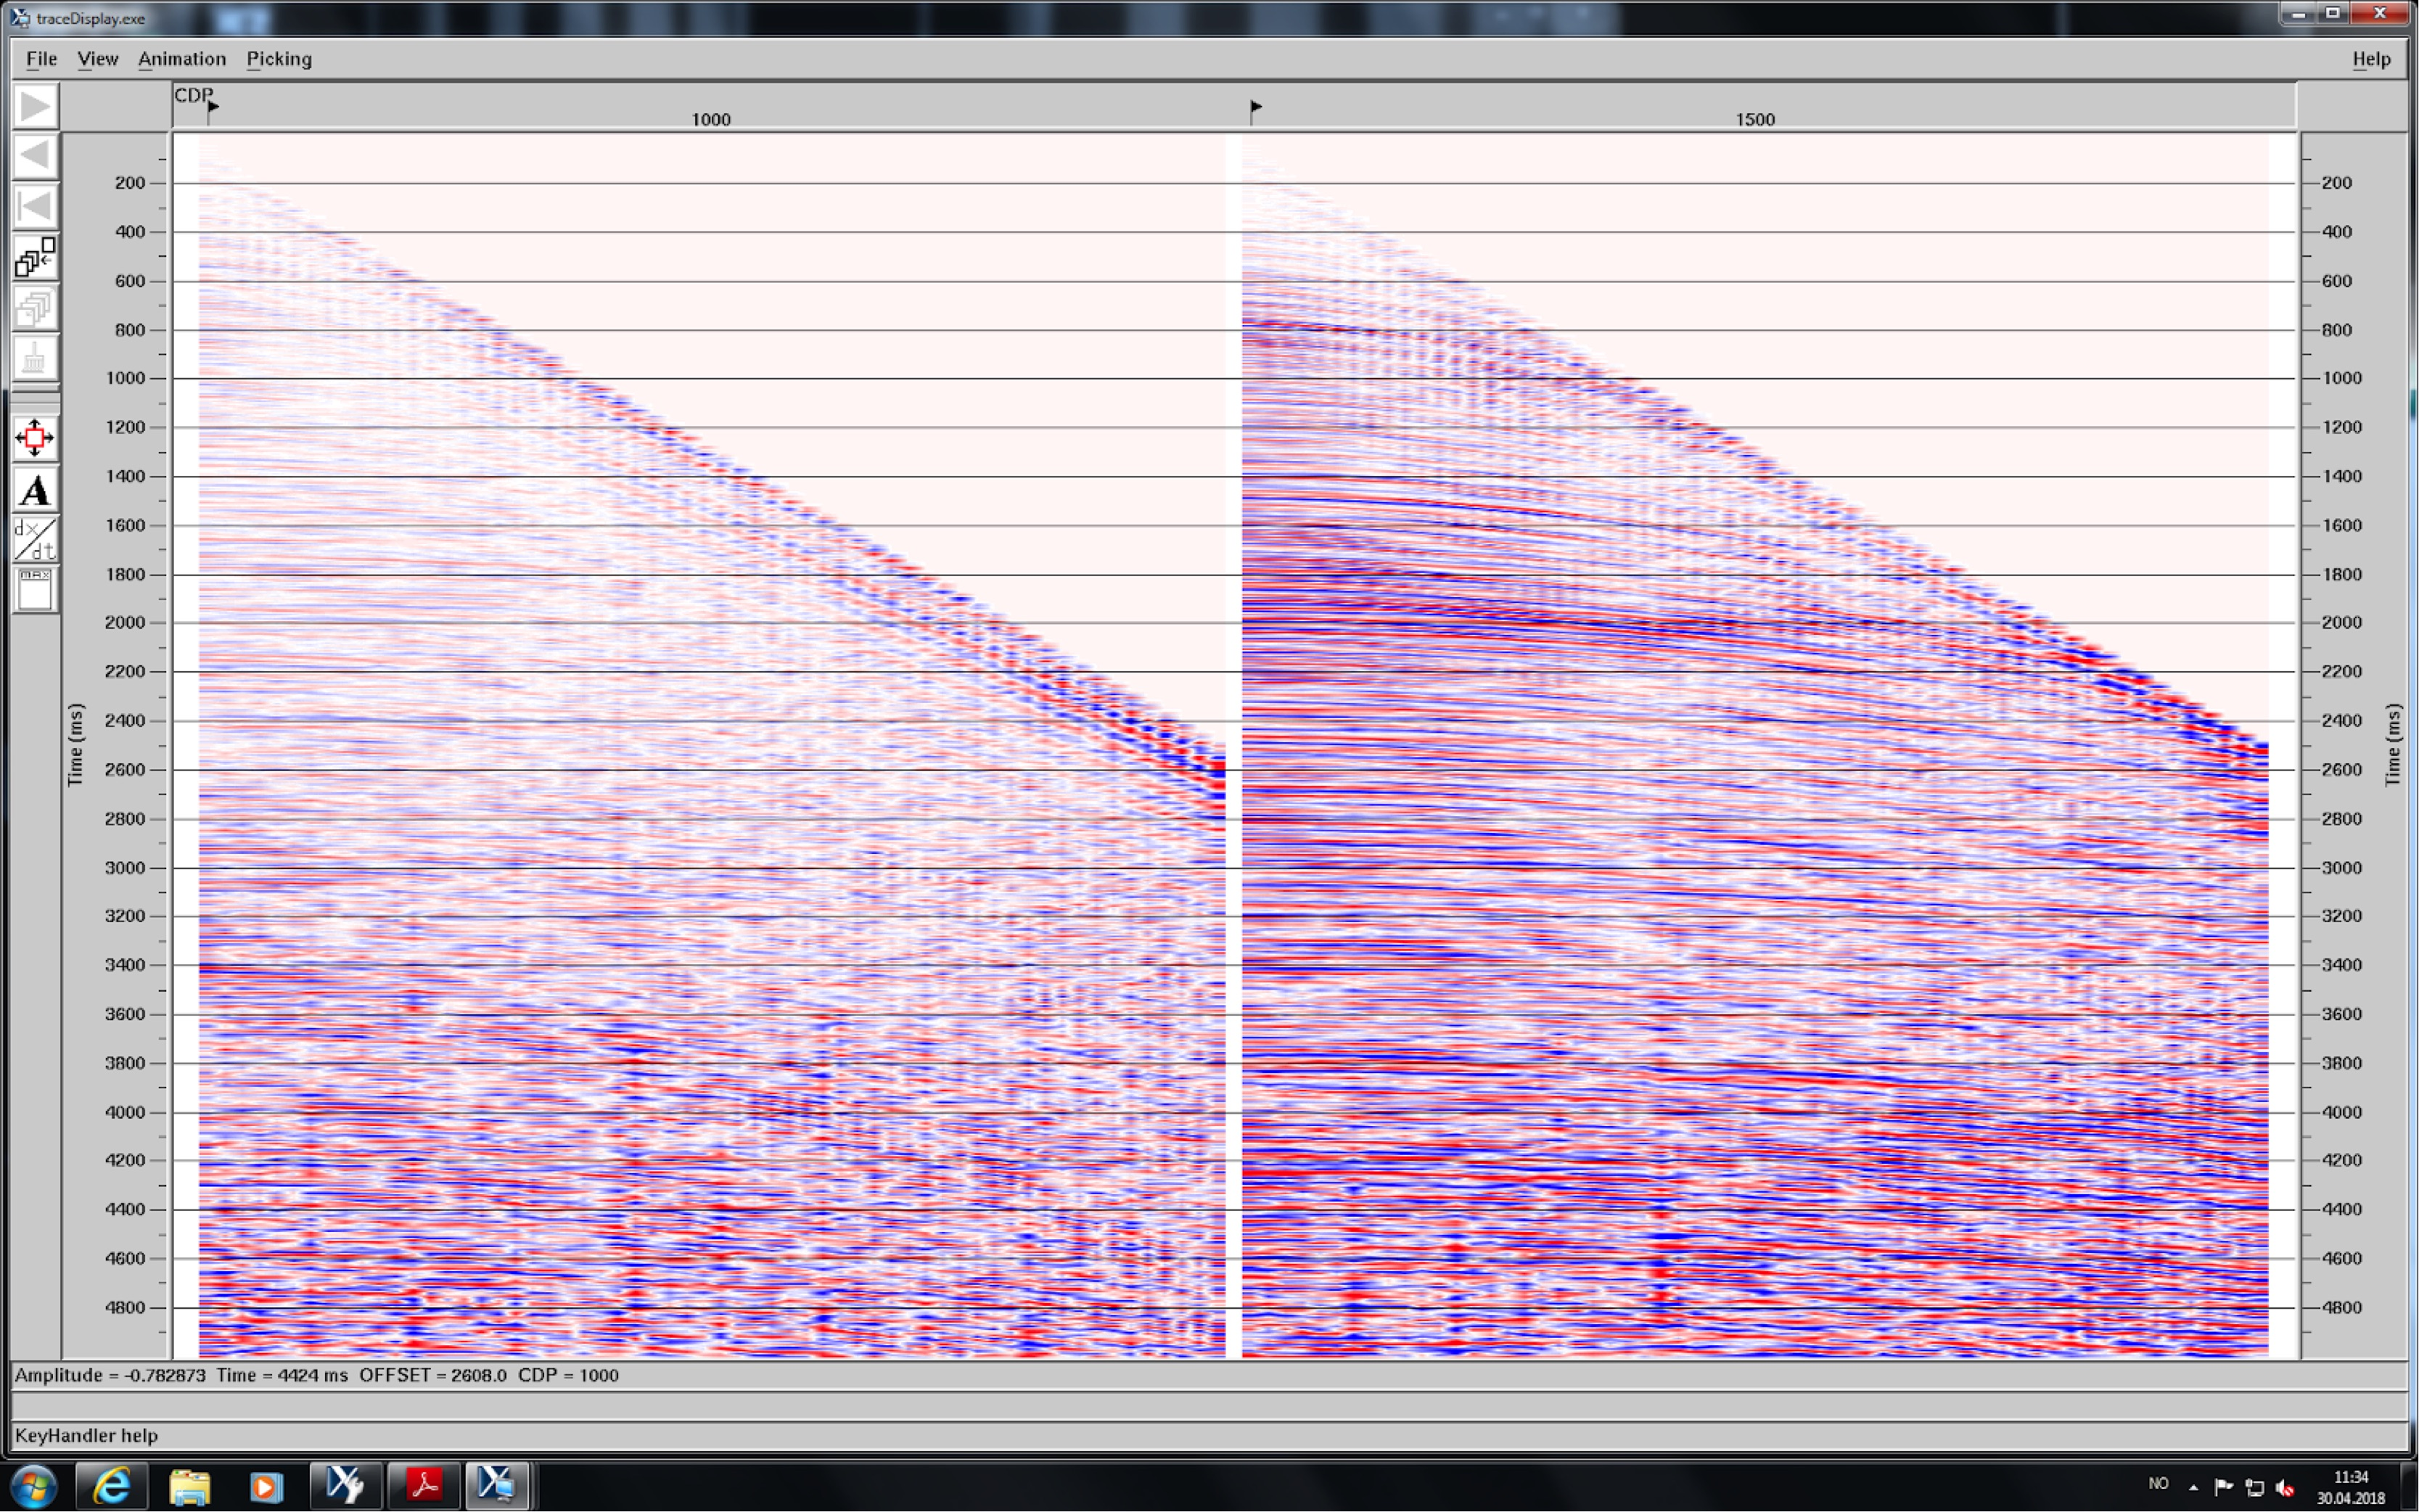
\includegraphics[width=\textwidth, trim={1.5cm 1.5cm 1cm 1.5cm},clip]{fig11.jpg}
\caption{CMP 1000 and 1500 after scaling, muting and also bandpass filtering by employing the Ormsby-filter.}
\label{fig11}
\end{figure}

\noindent Figure \ref{fig11} shows the data after bandpass filtering with a trapezoidal shape using filter [f1, f2, f3, f4] = [5, 10, 55, 65].
\\
Figure \ref{fig12} shows data in wiggle trace before and after bandpass filtering, figure \ref{fig13} - \ref{fig14} shows the effect in zoomed sections. The figures show improved imaging through removal of high and low frequencies deemed to be noise, leaving the main reflectors more visible.

\begin{figure}[H]
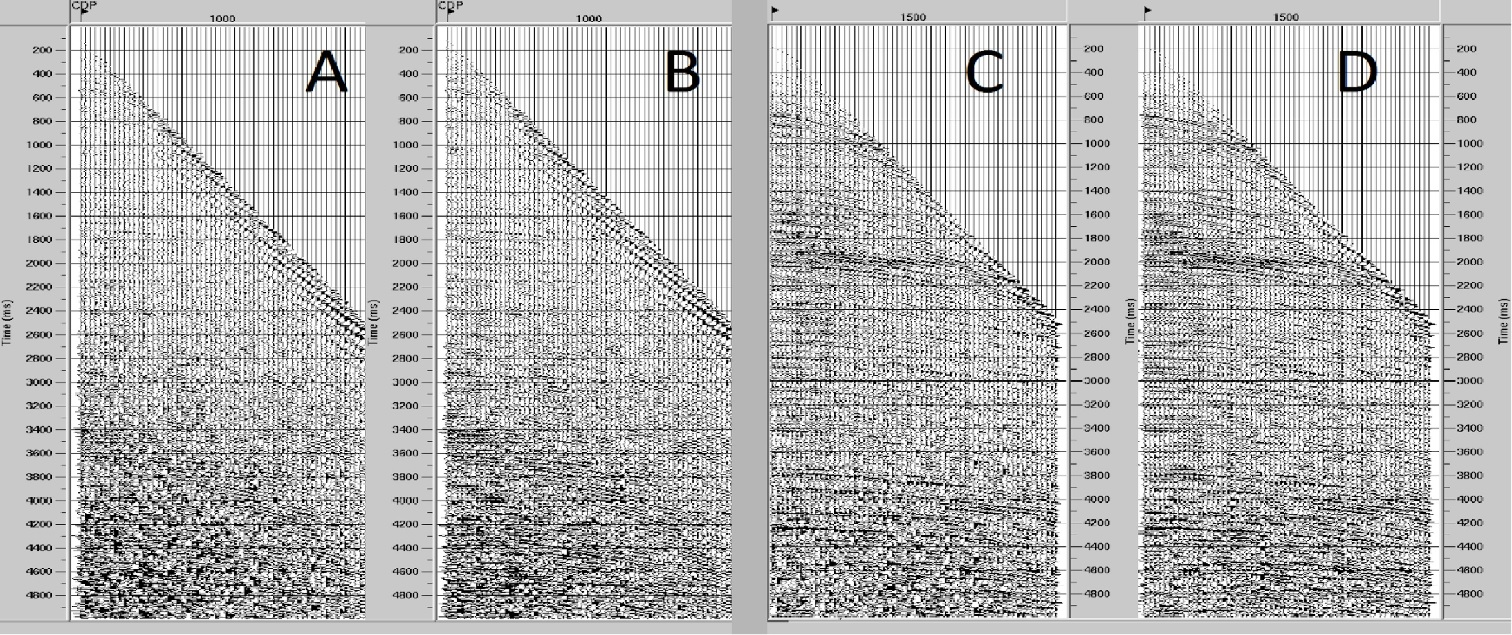
\includegraphics[width=\textwidth]{fig12.jpg}
\caption{CMP 1000 before (A) and after (B) bandpass filtering. CMP 1500 before (C) and after (D) bandpass filtering. Both are employing the Ormsby filter (described in detail in section 3.2).}
\label{fig12}
\end{figure}

\begin{figure}[H]
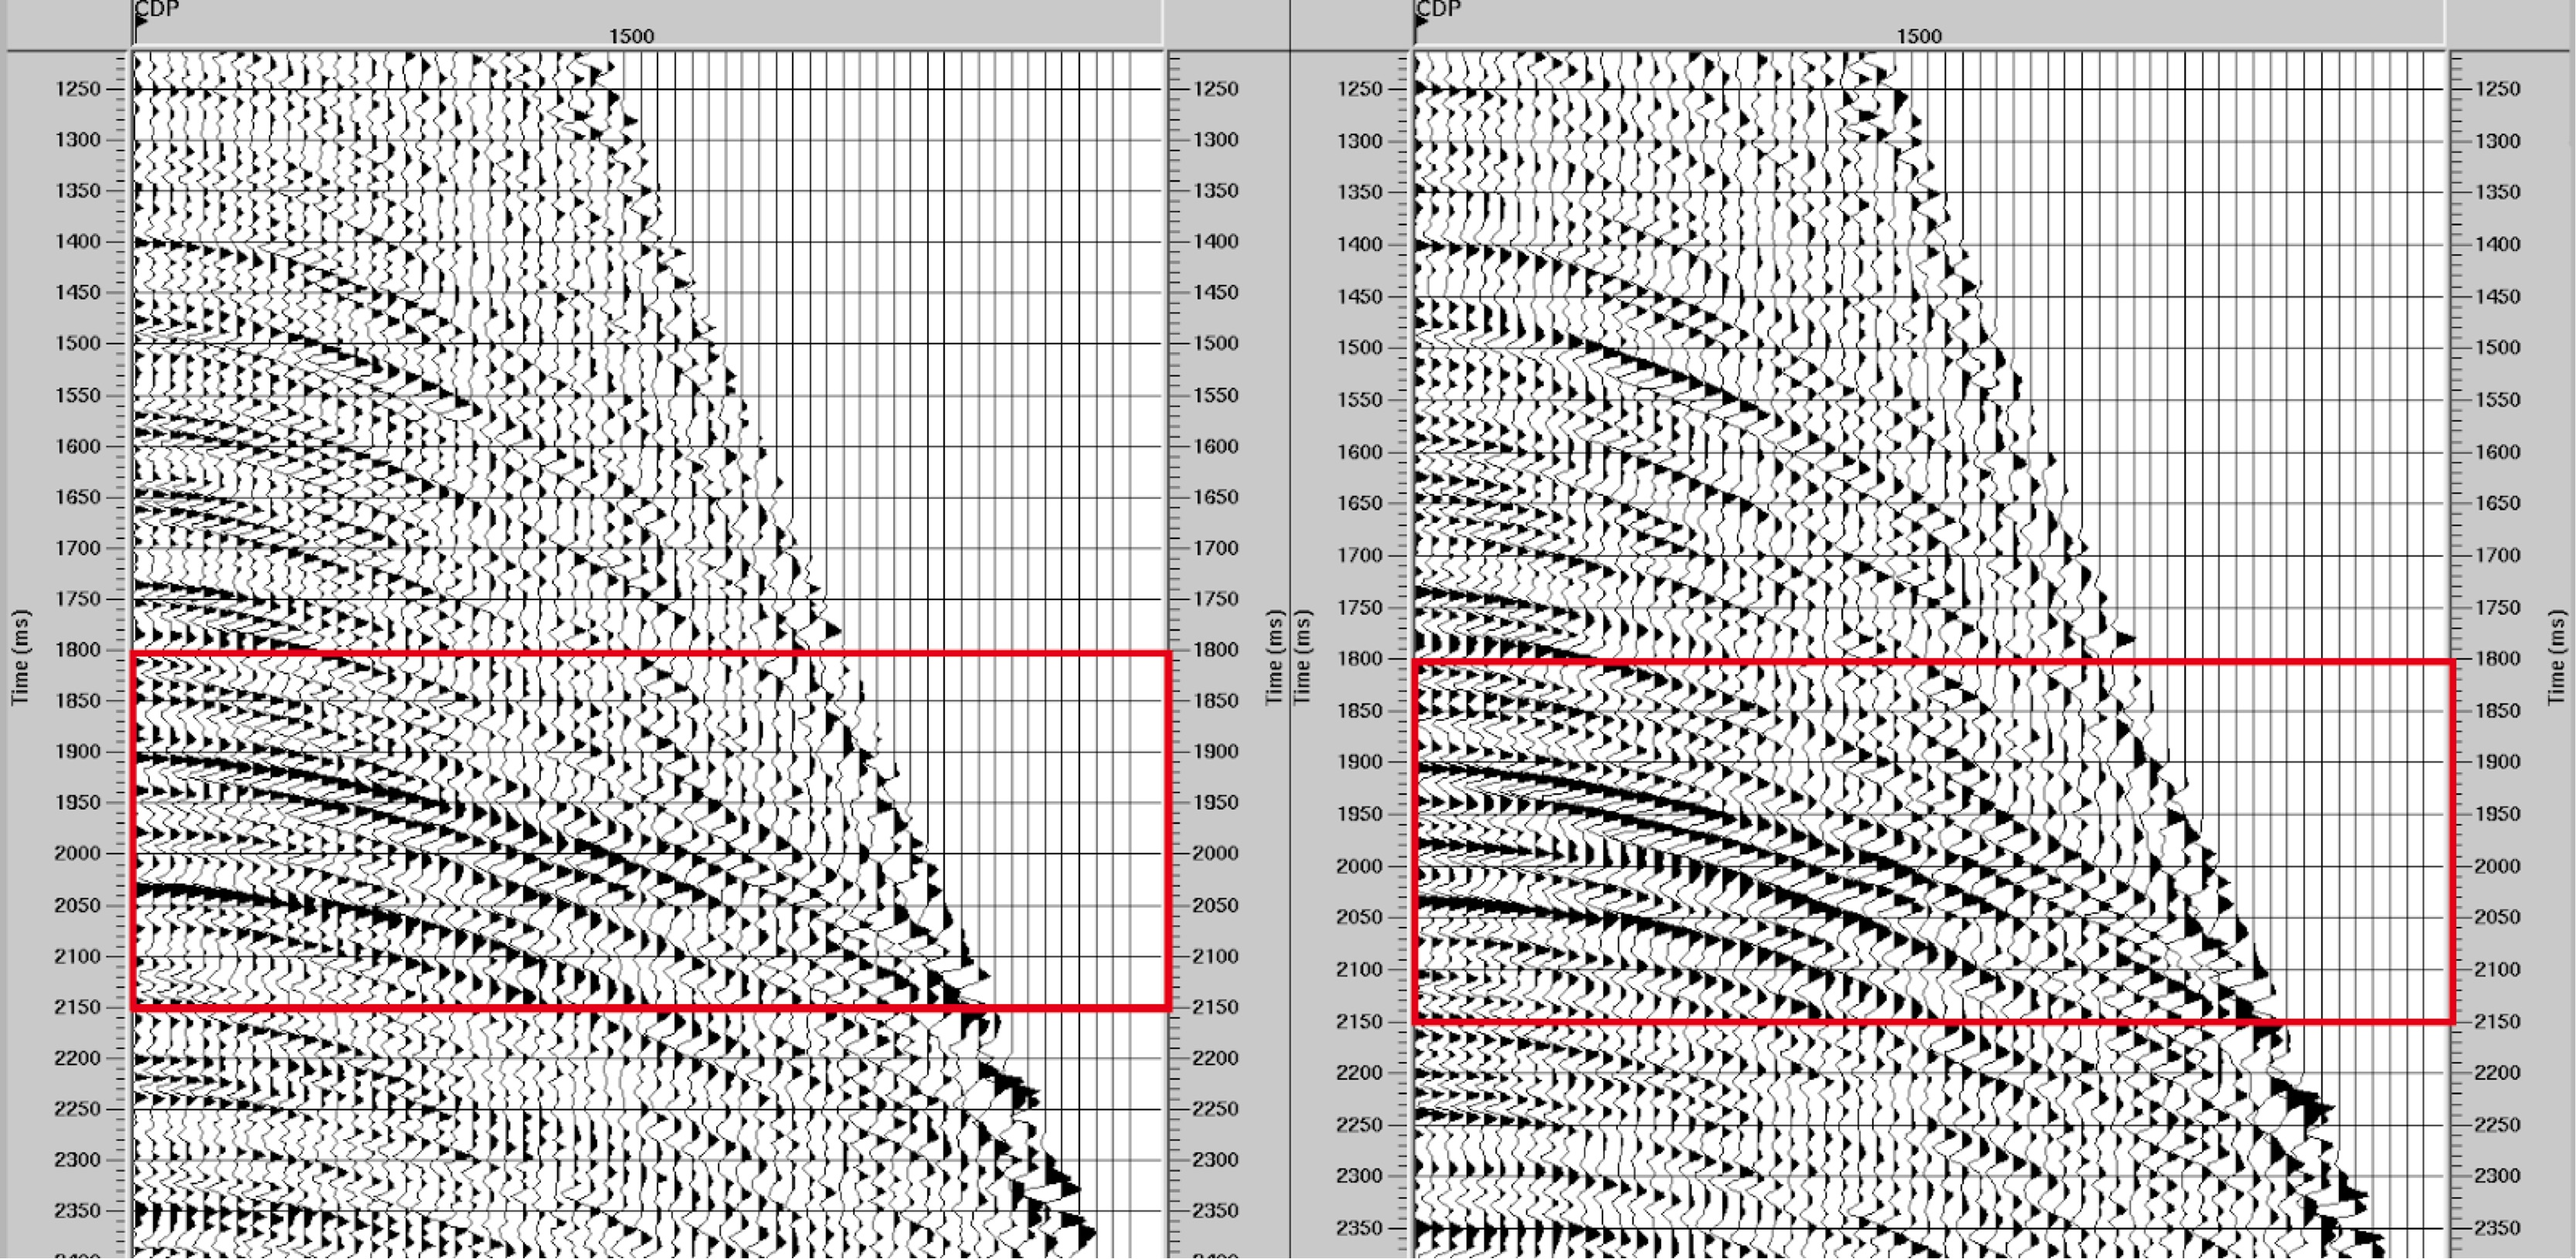
\includegraphics[width=\textwidth]{fig13.jpg}
\caption{Comparison of CMP 1500 before (left) and after (right) employing the Ormsby-filter, from traveltimes 1200 - 2400 ms. Areas with clearly visible effect is marked in red box, which also is displayed as zoomed section in figure \ref{fig14}.}
\label{fig13}
\end{figure}

\begin{figure}[H]
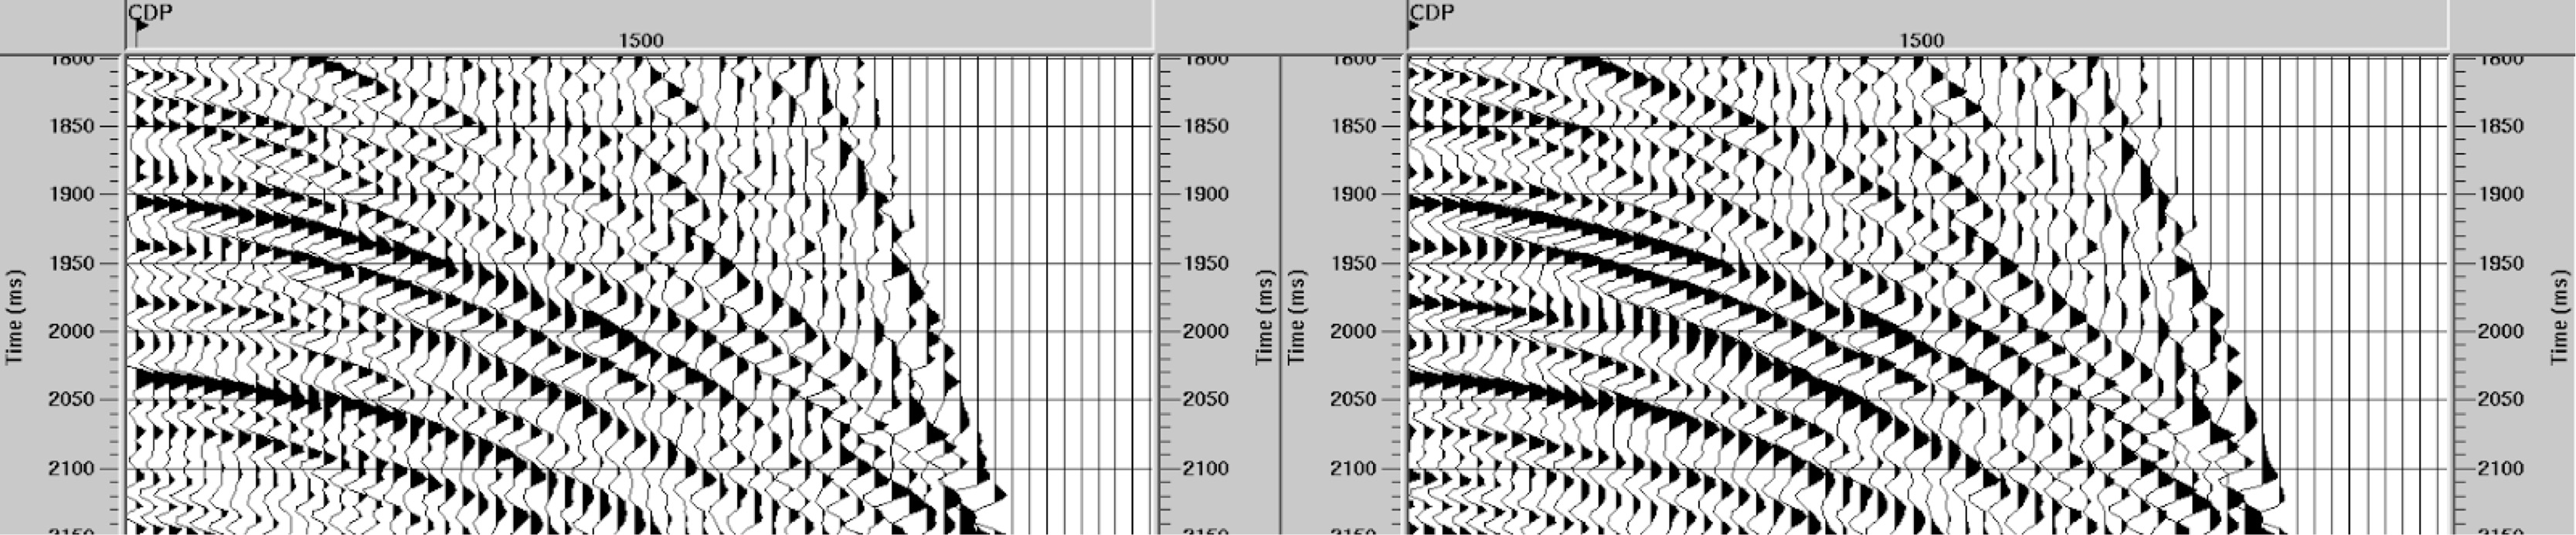
\includegraphics[width=\textwidth]{fig14.jpg}
\caption{Comparison of CMP 1500 before (left) and after (right) employing the Ormsby-filter, from traveltimes 1800 - 2150 ms. Notice better imaging after applying bandpass filtering through main reflectors becoming more prominent.}
\label{fig14}
\end{figure}

\subsection{Deconvolution and Autocorrelation}

A recorded seismic trace, x(t), can be described as a convolution of the source signal s(t) and the impulse response of the earth r(t).
$$
x(t) = s(t)*r(t)
$$

\noindent The goal of deconvolution is to identify an optimal filter, which after convolving with the data will give us the impulse response of the earth. These responses unfortunately contain reverberations, ghosts and multiples. Correlation provides a measurement of the similarity of two time-series. Auto-correlation compares the signal to itself, thus enhancing repetitions and simplifies detection of periodic signals, like multiples. During predictive deconvolution, auto-correlation is used to identify repetitive signals which are to be suppressed. This leads to improved quality of the data through increasing the S/N-ratio and thus imaging the subsurface with greater accuracy (Gelius, 2017a). 
\\
To perform predictive deconvolution one assumes that the seismic trace consists of a fully predictable part (e.g. periodic signals like multiples) and a fully non-predictable part (e.g. random reflectivity series). To distinguish these two parts of the seismic trace, a Wiener filter, a least-square filter method is used where the input signal consist of both primary and multiple pulses (n+$\alpha$). Predictive deconvolution estimates the contributions from multiples, $\alpha$, to further subtract these from the original data. Given an input wavelet of length (n+$\alpha$), the prediction error filter contracts it to an $\alpha$-long wavelet, where $\alpha$ is the prediction lag. 
\\
For this workflow CMP 1500 was autocorrelated for estimation of the multiple period. As deconvolution requires a vast amount of computing power, it was first tested on one CMP before applying it on all the CMPs. Convolution of the data was done by Ensemble Decon, which entails a single deconvolution operator being applied to groups of traces employing the predictive deconvolution.
\\
Figure \ref{fig15} and \ref{fig16} displays the autocorrelation without and with deconvolution of CMP 1500, respectively.


\begin{figure}[H]
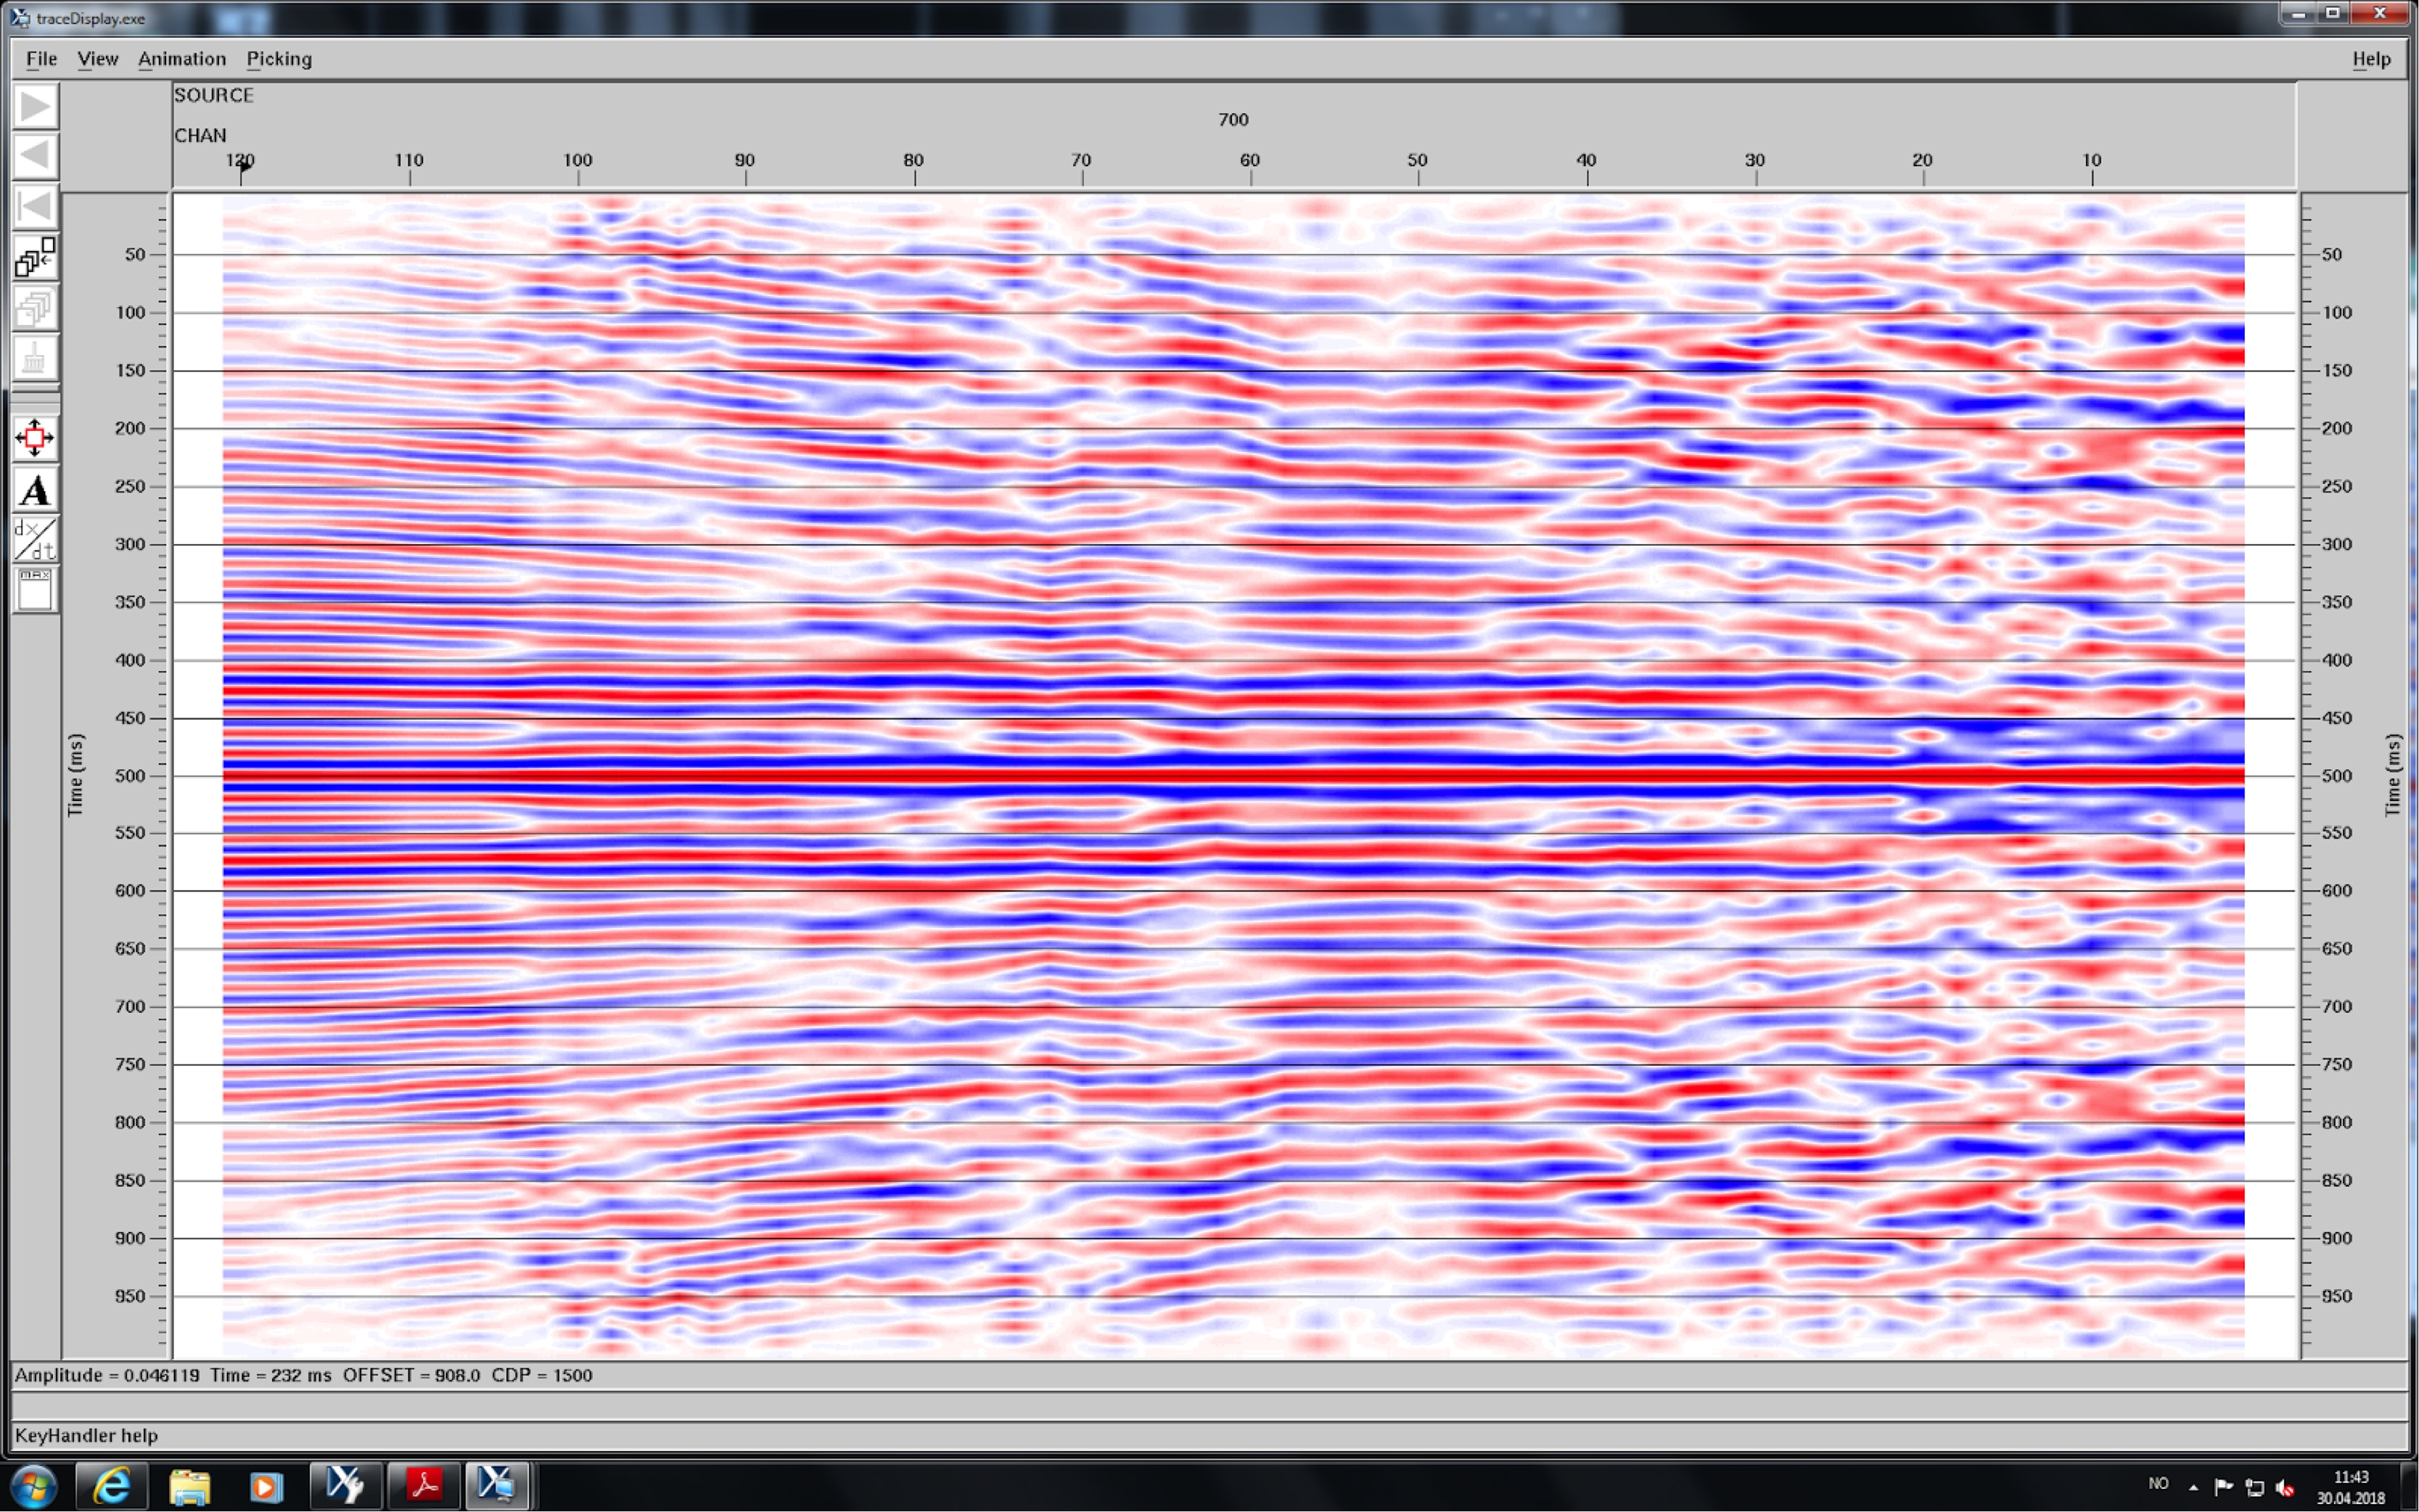
\includegraphics[width=\textwidth, trim={1.5cm 1.5cm 1cm 1.5cm},clip]{fig15.jpg}
\caption{Auto-correlation of CMP 1500 without applying deconvolution.}
\label{fig15}
\end{figure}

\begin{figure}[H]
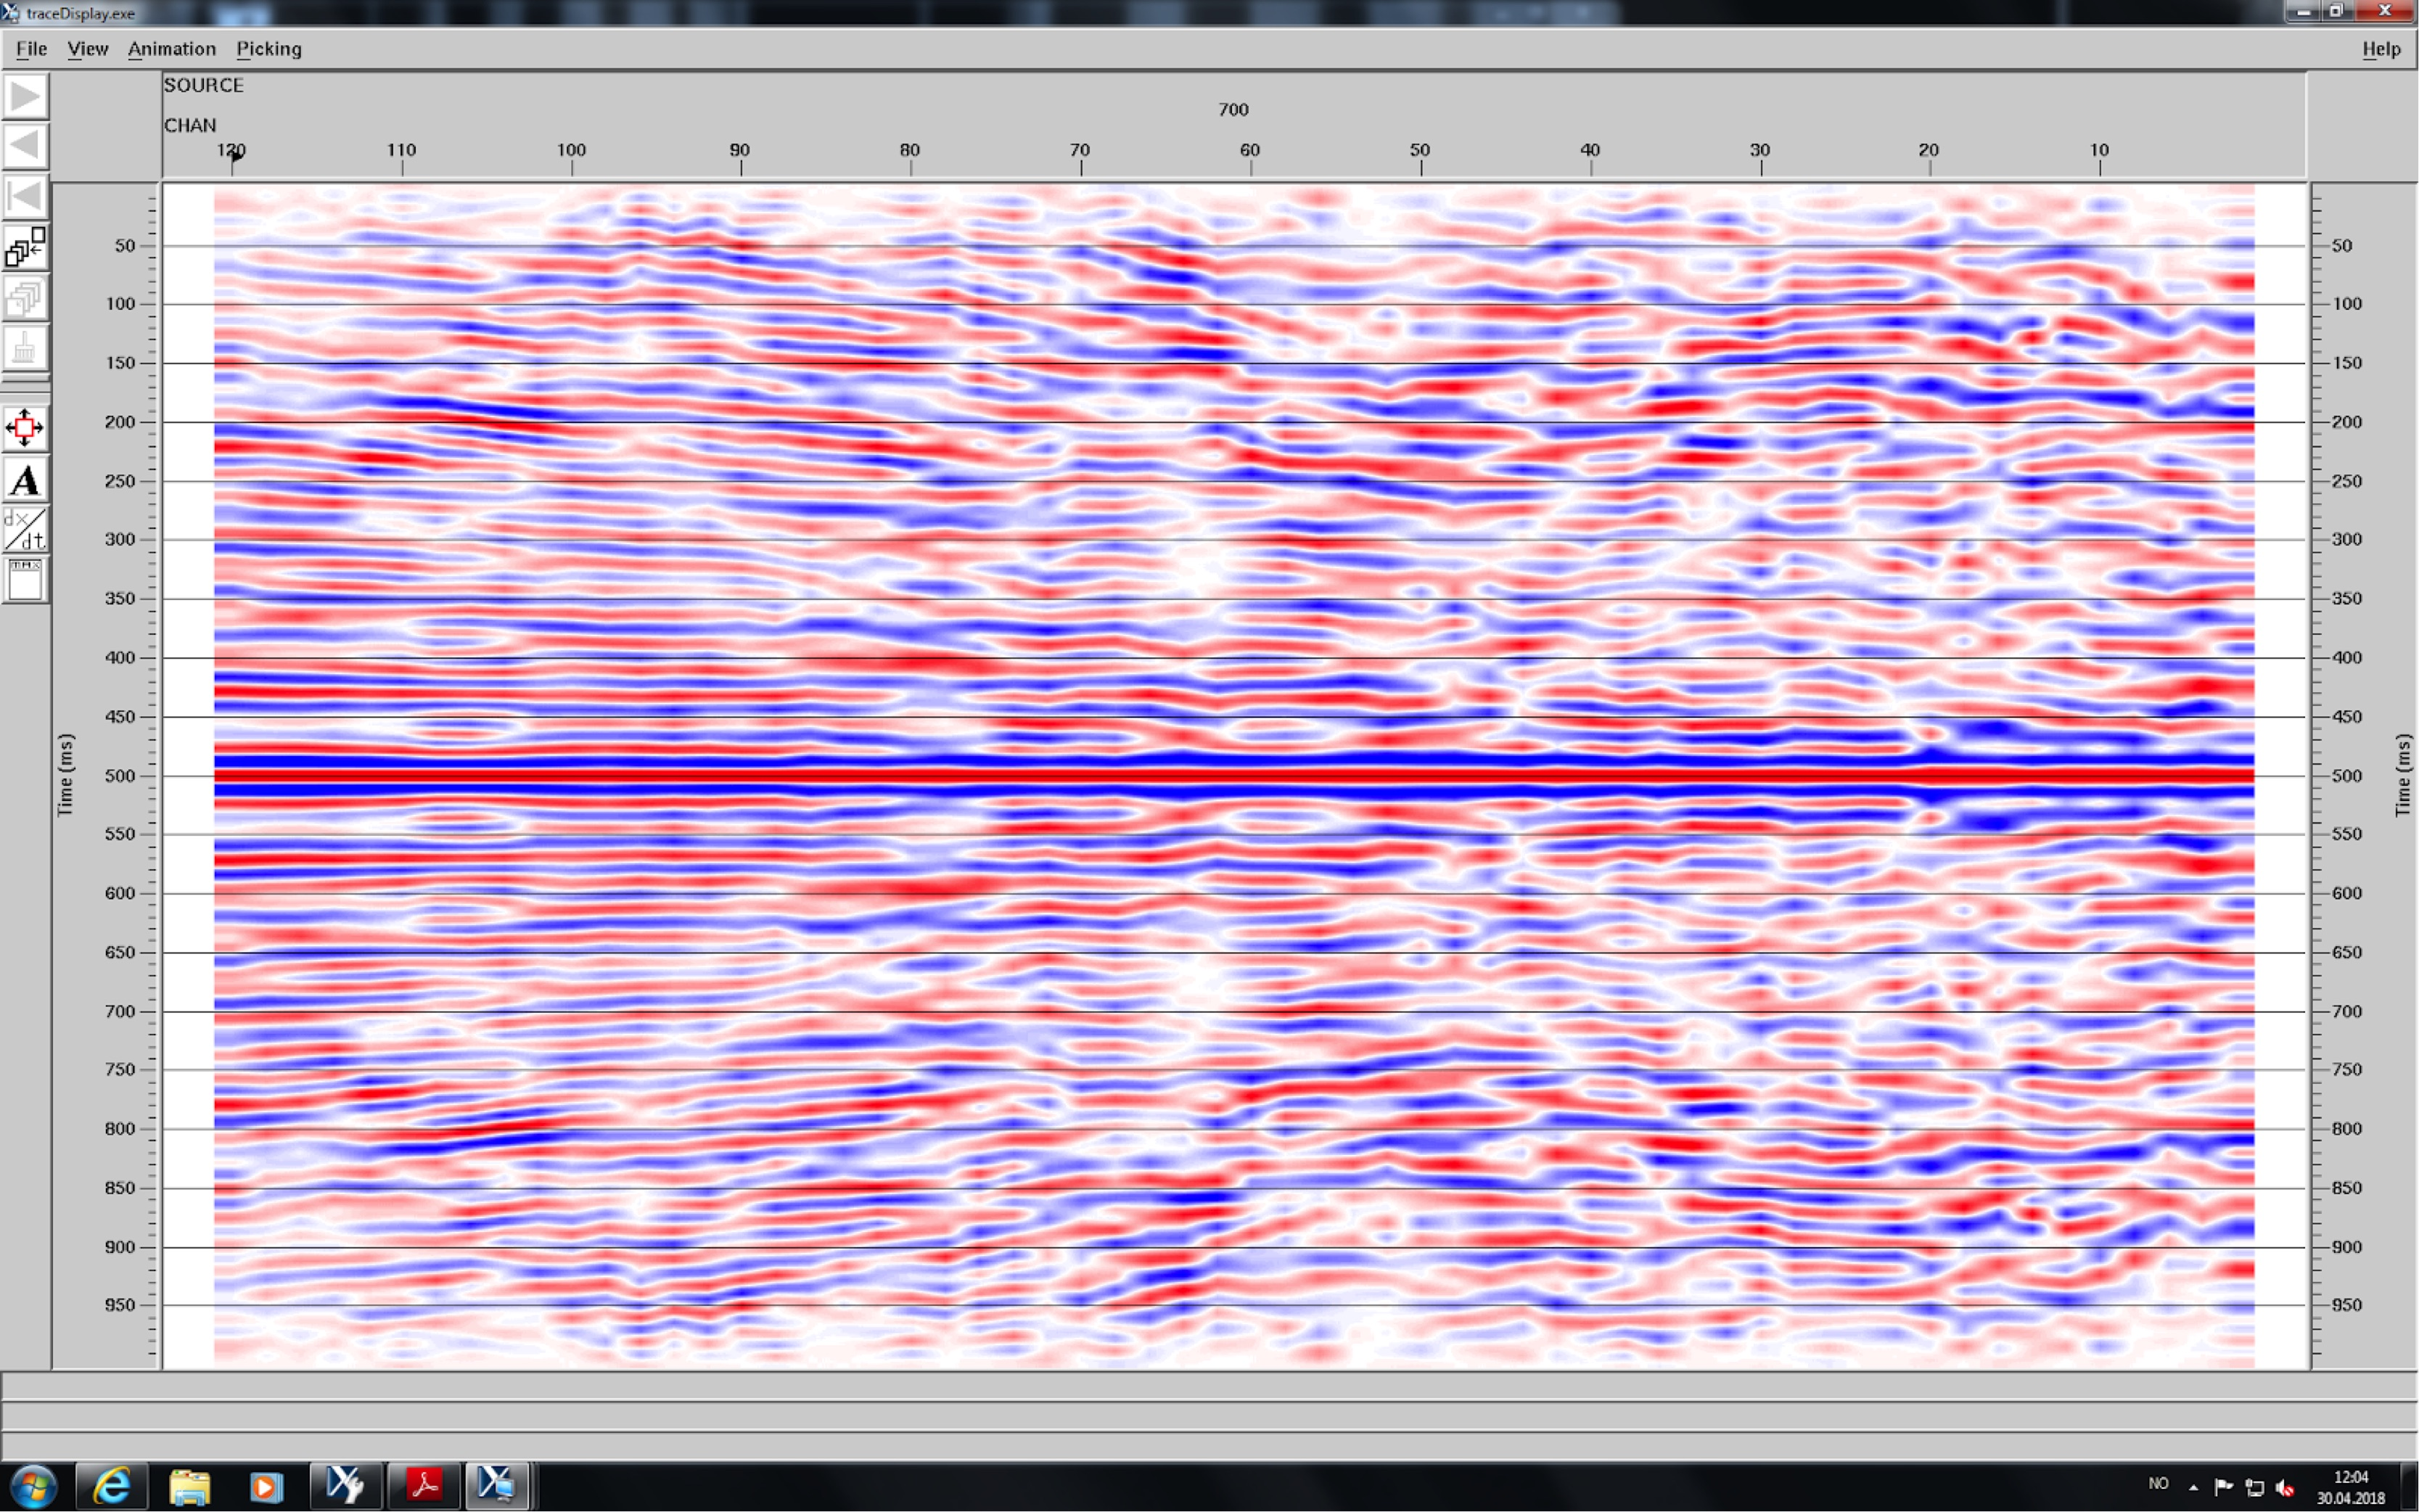
\includegraphics[width=\textwidth, trim={1.5cm 1.5cm 1cm 1.5cm},clip]{fig16.jpg}
\caption{Autocorrelation of CMP 1500 after applying deconvolution.}
\label{fig16}
\end{figure}

\noindent It is important to consider the polarity of the seismic data when considering sea bottom multiples. The polarity is determined by the change in acoustic impedance of the signal, corresponding to whether the reflection coefficient is of negative or positive value. As a calm sea surface gives a negative reflection coefficient -1 due to large impedance variations at this interface, this will cause a $180^{\circ}$ phase shift in associated multiples. Polarity change may be observed in the sea bottom multiples relative to the primary reflection, see figure \ref{fig17}. As polarity change is dependent on the reflection coefficient of the interface, not all multiples in the dataset will have a $180^{\circ}$ shift in polarity since the reflection coefficient of other interfaces are far from -1 (Gelius, 2018a).


\begin{figure}[H]
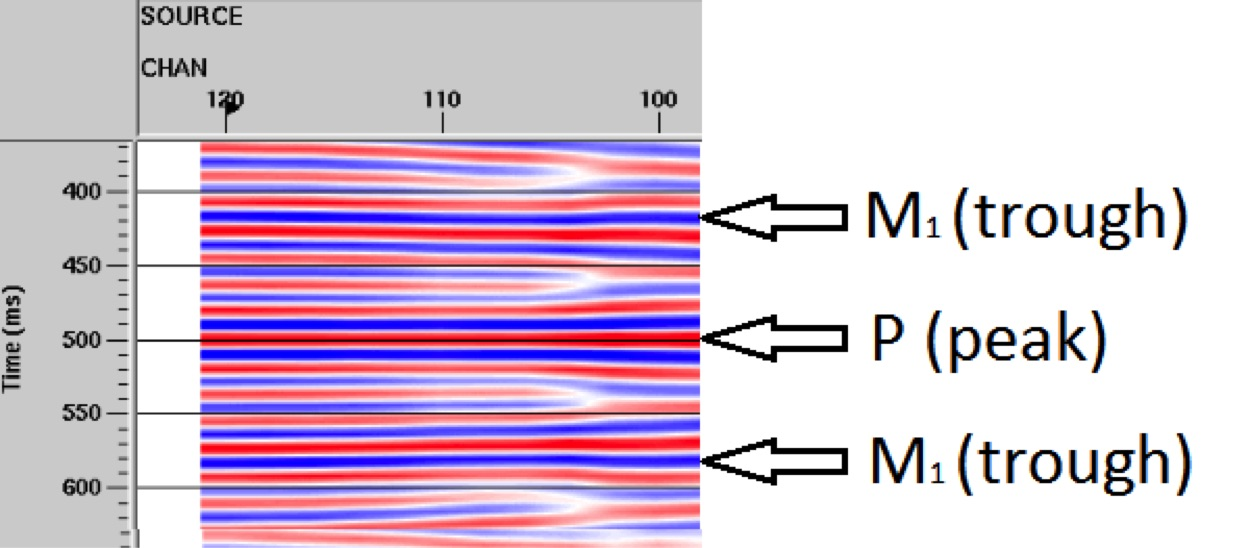
\includegraphics[width=\textwidth]{fig17.jpg}
\caption{Cut-out of times from 350 - 650 ms showing autocorrelation of CMP 1500, showing the primary reflector [P] (seafloor reflector) and the first multiples [M1]. As marked in the figure, the primary reflector has a positive reflection coefficient (peak) and the first multiples have negative reflection coefficient (troughs) due to phase change.}
\label{fig17}
\end{figure}

\noindent In comparing autocorrelation before and after performing deconvolution, see figures \ref{18}-\ref{20}, the primary reflector is evidently clearer and multiples are almost undetectable, proving autocorrelation and deconvolution having a prominent positive effect in imaging by increasing the S/N-ratio (as the multiples are to be recognized as noise).

\begin{figure}[H]
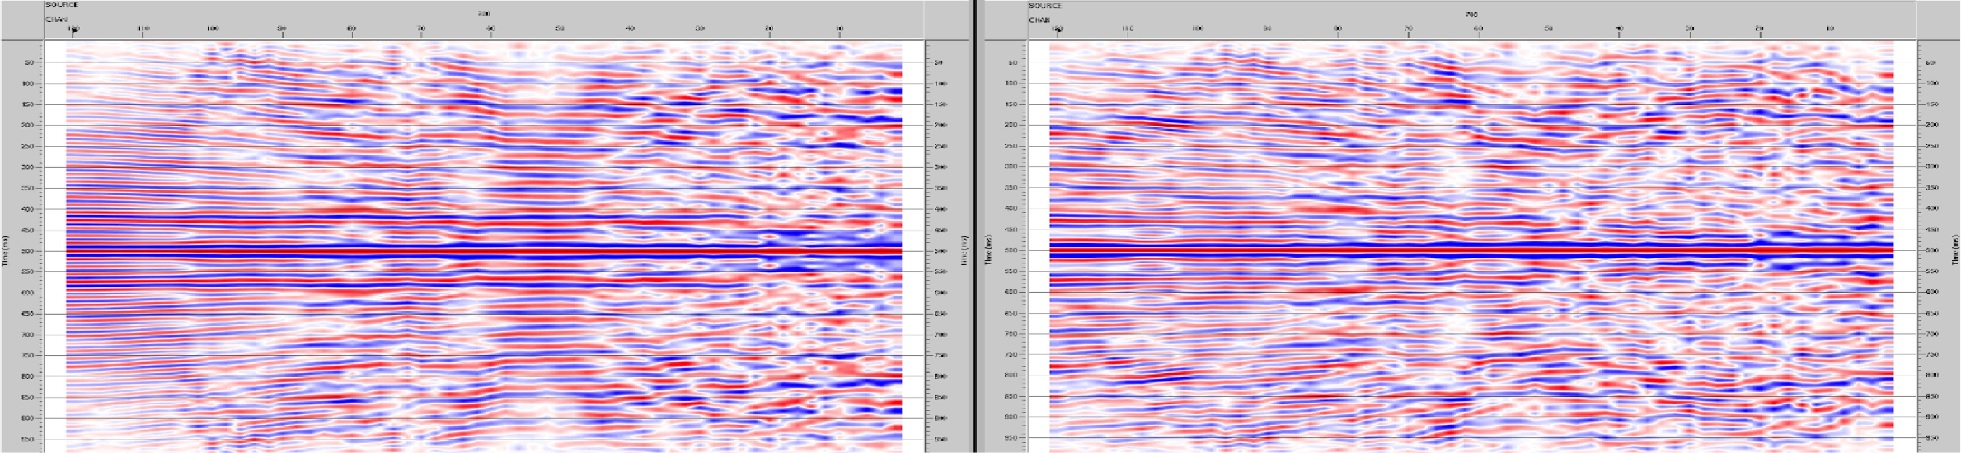
\includegraphics[width=\textwidth]{fig18.jpg}
\caption{Comparison of the autocorrelation of CMP 1500 before (left) and after (right) deconvolution has been applied. Notice the increased clarity of the primary reflector and the reduction of the multiples.}
\label{fig18}
\end{figure}

\begin{figure}[H]
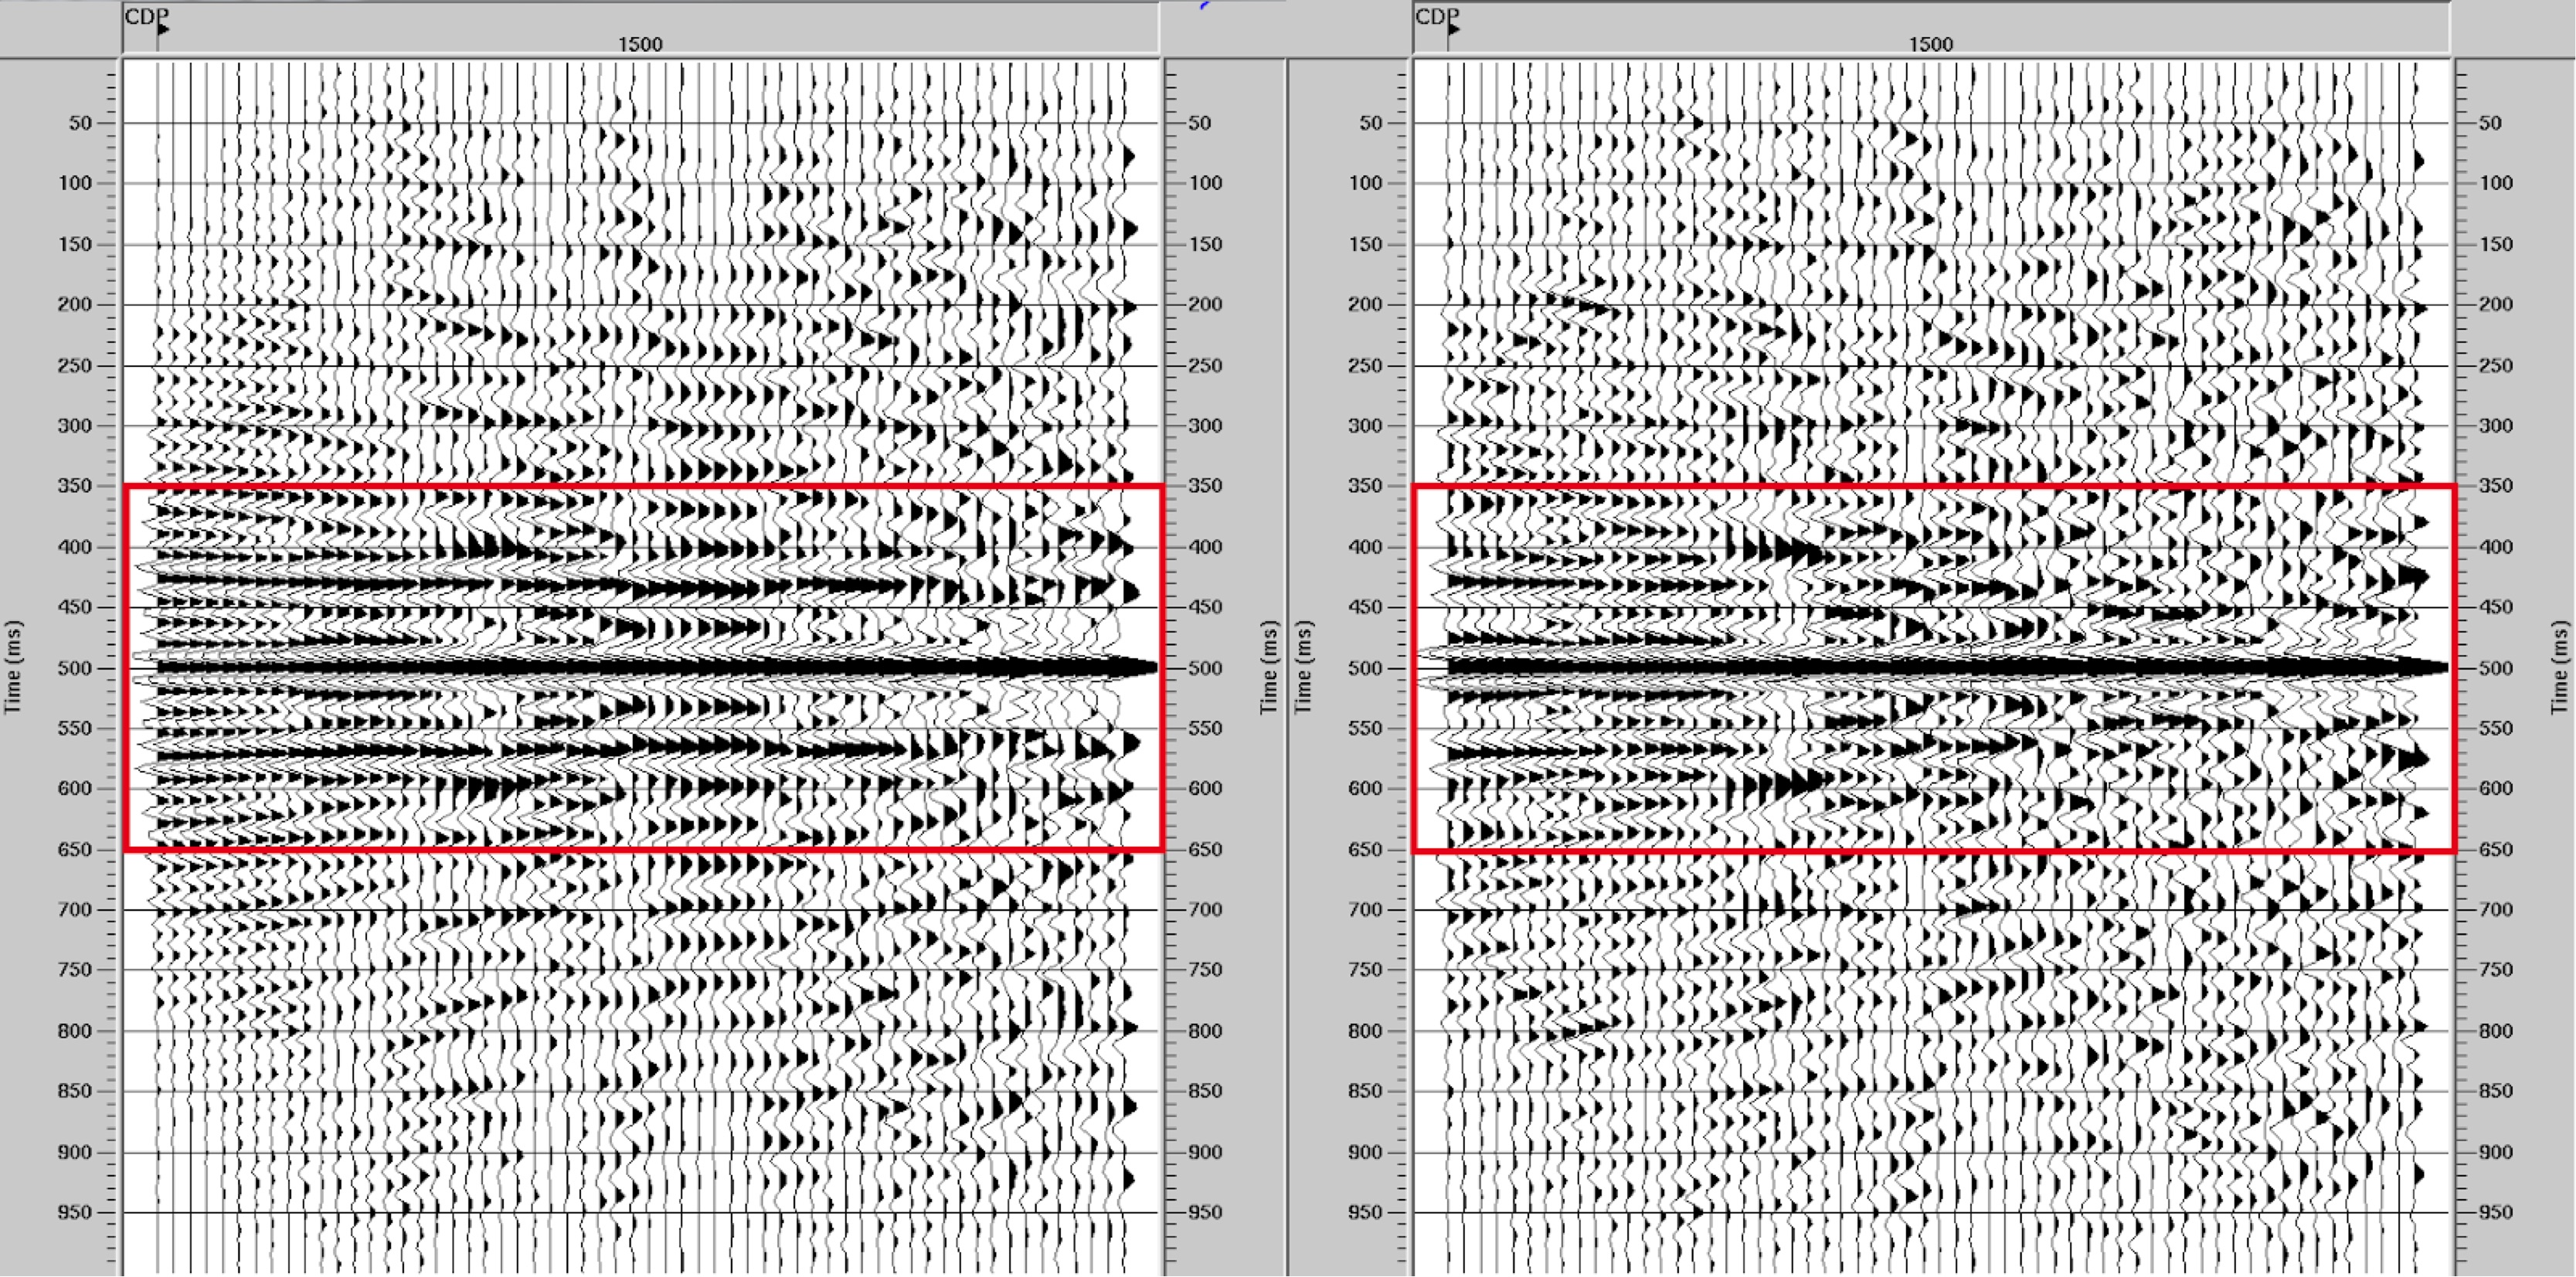
\includegraphics[width=\textwidth]{fig19.jpg}
\caption{CMP 1500 before (left) and after (right) deconvolution. Notice how multiples are heavily reduced during deconvolution.}
\label{fig19}
\end{figure}

\begin{figure}[H]
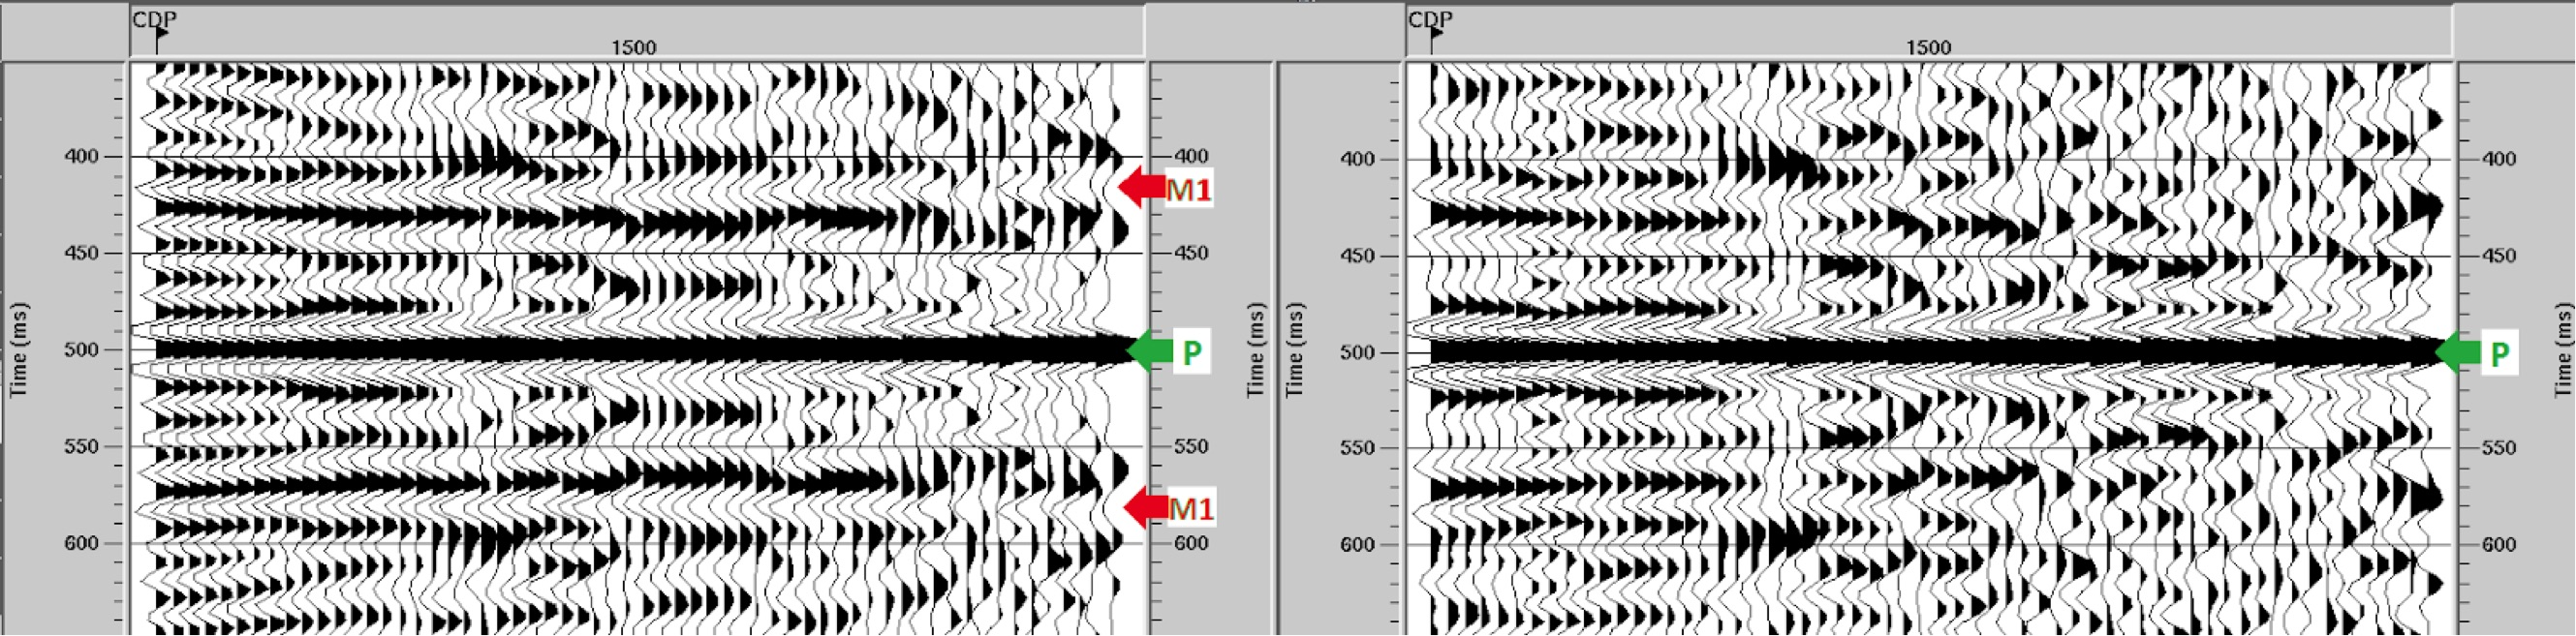
\includegraphics[width=\textwidth]{fig20.jpg}
\caption{Cut-out of times from 350 - 650 ms showing autocorrelation of CMP 1500 before (left) and after (right) deconvolution. Multiples [M1] are marked with red arrows, Primary reflector [P] is marked with green arrow. (Zoomed section of red box in Figure \ref{fig19})}
\label{fig20}
\end{figure}


\section{Velocity Analysis, NMO-correction and Stacking}

\subsection{Velocity Analysis}

Prior to stacking, NMO-correction need to be applied to the different gathers. To ensure the most accurate NMO-corrections, a velocity analysis is performed. The chosen velocity is called the stacking velocity, which forms the basis for the velocity model. Employing a good velocity model creates a good basis for stacking, and thus also accurate travel time-depth conversion and migration (Baird Petrophysical, 2005).
\\
The analysis consists of trying to determine the velocity distribution through the the model as a function of time (ProMAX, 2018; Gelius, 2018a). When fitting the data into a NMO-velocity model one assumes a horizontally layered earth model, and that the offsets are small spread. All offsets in the CMP-gather are used with intent to fit the reflections to an optimal hyperbolic traveltime model (Gelius, 2018a). 
\\
Correcting and stacking CMP-data for many different velocities within discrete time windows repeatedly is a common form of velocity analysis. As a general rule, the guiding velocity function is picked to go through areas with the highest semblance values (Gelius, 2018a).
\\
During this workflow, velocity analysis was performed on 12 equally spaced CMPs over the entire model. It was carried out by manually picking velocities using the semblance panel, with intent to generate the optimal correction of the CMP-gather resulting in horizontal primary reflectors. Picking velocities involve choosing points in the semblance panel with as high semblance values as possible without deviating excessively from the provided velocity guide function. Implicitly, this assumes meagre lateral variations in geology, coinciding with the velocity functions being calculated assuming small variations in velocity change. The manually picked velocities on the 12 CMPs are further interpolated between these gathers.
\\
Striving for as high semblance as possible consequently minimizes risk of over- or undercorrection. If velocities are too high, this leads to undercorrection of the reflectors causing the reflectors to curve downwards. On the other hand, if velocities are too low, this causes upwards curvature due to overcorrection of the reflectors, see figure \ref{NMOoverunder}.

\begin{figure}[H]
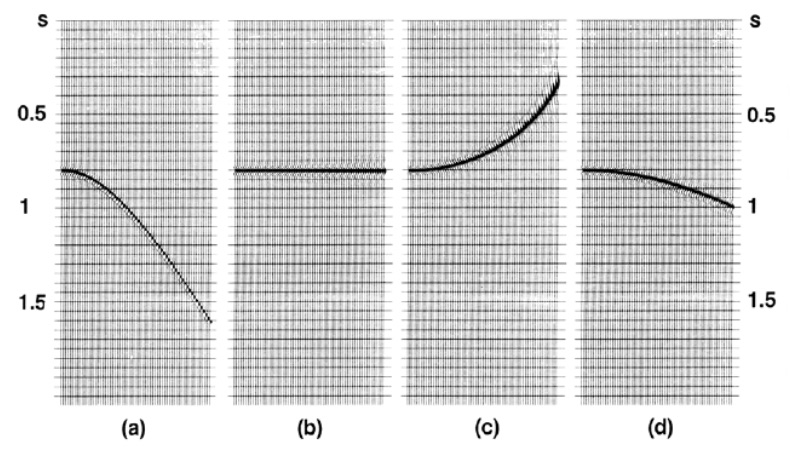
\includegraphics[width=\textwidth]{NMOcorr_over_under.jpg}
\caption{Illustration of over and under-corrected traces. (a) and (d) are under-corrected, (b) is perfectly corrected and (c) is over-corrected}
\label{NMOoverunder}
\end{figure}

\noindent Velocity analyses for CMP 870 and CMP 1190 can be seen in figures \ref{VA870} - \ref{VA1190}, where the panels (from the left) are the:

\begin{enumerate}
    \item Velocity spectrum/semblance panel: showing variations in velocities and their semblance to the velocity model. The highest semblance is marked with red colour
    \item Gather panel: CMP, time vs. offset
    \item Dynamic stackpanel: showing mini-stacks based on the velocities picked using the semblance panel
    \item Function stack panel: showing mini-stacks based on one single velocity function with a constant velocity (constant velocity stacks) (Gelius, 2018a; ProMax, 2018)
\end{enumerate}

\begin{figure}[H]
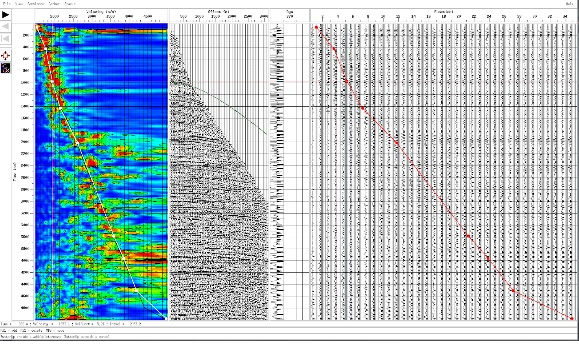
\includegraphics[width=\textwidth]{Velo_anal_870.jpg}
\caption{Velocity analysis for CMP 870. Four columns, respectively representing from the left: semblance panel, gather panel, dynamic stack panel and function stack panel.}
\label{VA870}
\end{figure}

\begin{figure}[H]
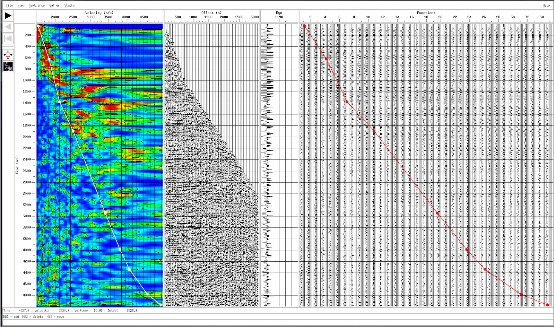
\includegraphics[width=\textwidth]{Velo_anal_1190.jpg}
\caption{Velocity analysis for CMP 1190. Four columns, respectively representing from the left: semblance panel, gather panel, dynamic stack panel and function stack panel.}
\label{VA1190}
\end{figure}

\noindent The result of the velocity analysis and corresponding NMO correction for CMP 870 and 1190 are shown in figure \ref{NMO870} - \ref{NMO1190}.

\begin{figure}[H]
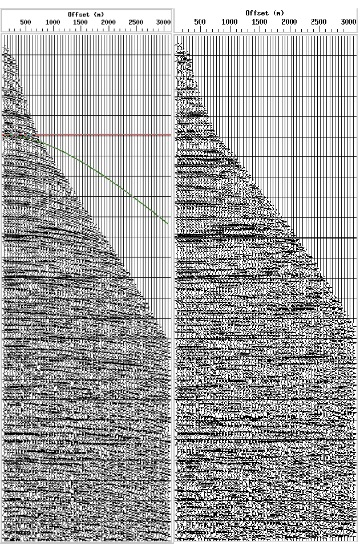
\includegraphics[width=\textwidth]{beforeAfter_NMOcorr_870.jpg}
\caption{Comparison of CMP 870 (gather panels) before (left) and after (right) applied NMO-correction. Notice how the reflections have more of a horizontal trend after applying NMO-correction.}
\label{NMO870}
\end{figure}

\begin{figure}[H]
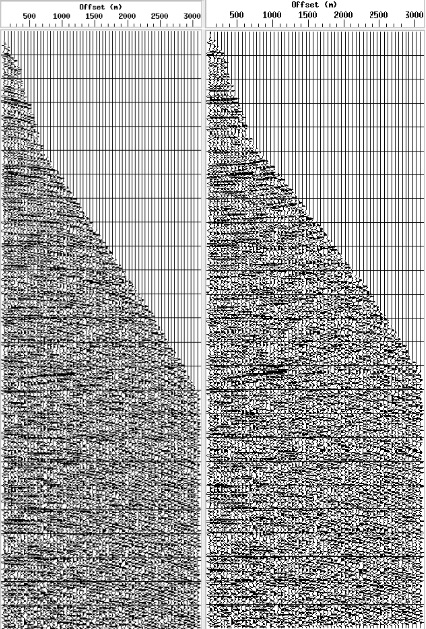
\includegraphics[width=\textwidth]{beforeAfter_NMOcorr_1190.jpg}
\caption{Comparison of CMP 1190 (gather panels) before (left) and after (right) applied NMO-correction. Notice how the reflections have more of a horizontal trend after applying NMO-correction.}
\label{NMO1190}
\end{figure}

\noindent Satisfactory alignment of the traces may be seen at low offsets, indicating successful NMO. At increasing offsets however, the NMO-correction seems less accurate and tendencies of over and undercorrection may be observed, see figures \ref{VA870ex} - \ref{VA1190ex}.

\begin{figure}[H]
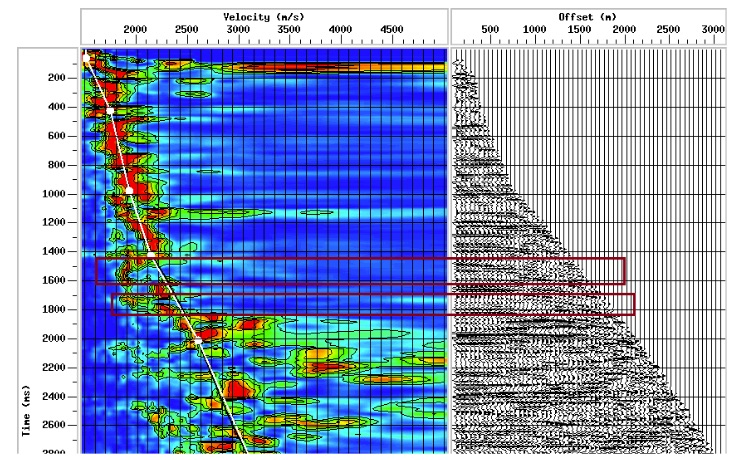
\includegraphics[width=\textwidth]{Velo_anal_example_870.jpg}
\caption{Semblance panel and gather panel for CMP 870. Intervals where the velocity model has greater velocities than those in the semblance map are boxed in, along with the coinciding undercorrected reflectors, dipping slightly downwards seen in the gather panel.}
\label{VA870ex}
\end{figure}

\begin{figure}[H]
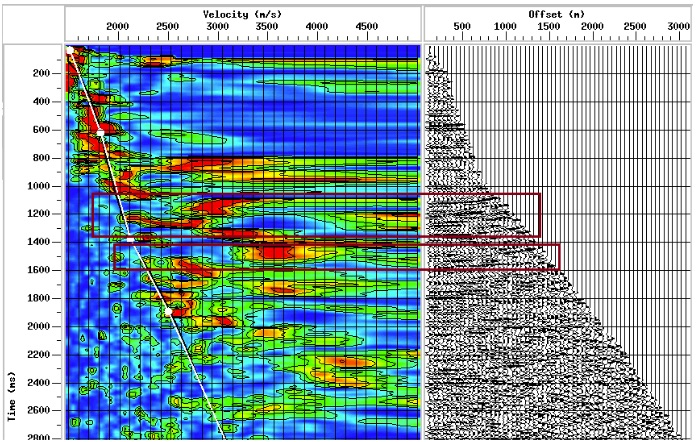
\includegraphics[width=\textwidth]{Velo_anal_example_1190.jpg}
\caption{Semblance panel and gather panel for CMP 1190. Intervals where the velocity model has lower velocities than those in the semblance map are boxed in, along with the coinciding overcorrected reflectors, dipping slightly upwards seen in the gather panel.}
\label{VA1190ex}
\end{figure}

\subsection{Velocity Analysis Quality Control}

As the velocity analysis was performed using the CMP-method, the analysis assumes a geological model corresponding to a velocity field that gradually varies as a function of traveltime without any significant lateral variations. If these assumptions prove incorrect both the velocity analysis and the stacked section may be distorted. Such anomalies might be caused by diffractions, multiples, shallow gas pockets, interference, dip and out-of-plane reflections (Gelius, 2018a). 

\begin{figure}[H]
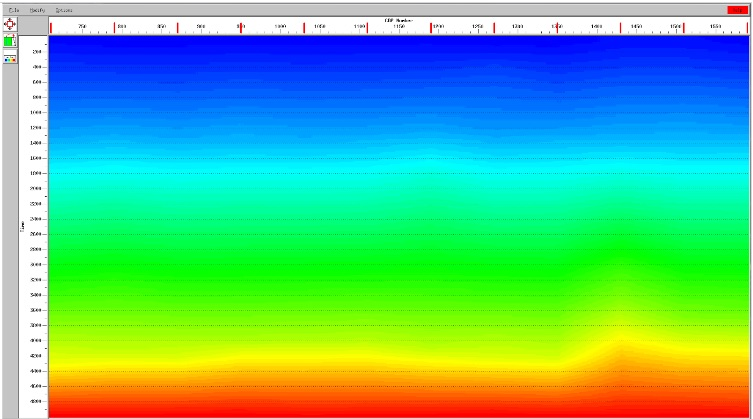
\includegraphics[width=\textwidth]{Velo_anal_smooth.jpg}
\caption{The result from the velocity analysis. Velocity is clearly increasing with travel time, but there are some irregularities.}
\label{Smooth}
\end{figure}

\noindent Figure \ref{Smooth} shows the result of the velocity control, displaying the velocity field. As the field shows no significant signs of abrupt distortions or lateral variations the field may be applied when NMO-correcting the data.


\subsection{NMO-correction and Stacking}

Successive shots in a marine CMP-gather increases travel time for the respective seismic waves between source and receiver, which is reflected in the delay of the seismic traces. The additional traveltime are called normal moveout (NMO) and this must be corrected for, see figure \ref{NMOS}.

\begin{figure}[H]
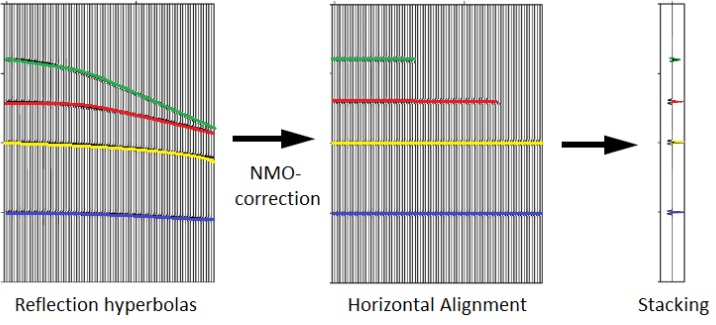
\includegraphics[width=\textwidth]{NMOcorr_stacking.jpg}
\caption{Illustration of how NMO-correction and stacking works in theory. The traces are aligned at different offsets and then added together in the stacking process.}
\label{NMOS}
\end{figure}

\noindent The NMO-correction effectively repositions the traces to a lower TWT at the different offsets. The amount of repositioning is determined by the equation where the $v_{nmo}$ is identified by velocity analysis:
$$
\Delta t = t(x) - t_0 = \sqrt{t_0^2 + \frac{x^2}{v_{nmo}^2}}-t_0
$$

This equation holds two major assumptions:

\begin{itemize}
    \item A flat earth model (no dip correction)
    \item Small offsets
\end{itemize}

\noindent From the equation above, one may observe that a too large $v_{nmo}$ results in too small of a correction and vice versa, as previously illustrated in figure \ref{NMOoverunder}. If the $v_{nmo}$, and therefore the correction, is wrongly calibrated, the reflectors will not align when stacked resulting in seismic section without any clear interfaces. 
\\
Given a constant velocity $v_{nmo}$ and offset x, the correction $\Delta t$ becomes smaller when $t_0$ becomes larger. NMO is also non-linear with respect to offset and travel time. This tells us that the correction is far from constant along a trace, and the correction becomes more extrusive for larger offset or shallow depths with lower velocity. This leads to NMO-stretching. These stretches are easily muted after the NMO-correction.
\\
Stacking is then performed on the NMO-corrected traces in the CMP-gathers. The result of the stacking is thus dependant on the quality of the velocity analysis.

\section{Migration}

After muting, scaling, filtering, autocorrelation and deconvolution, velocity analysis, NMO-correction and stacking the result is a post-stack non-migrated section, see figure \ref{fmig}

\begin{figure}[H]
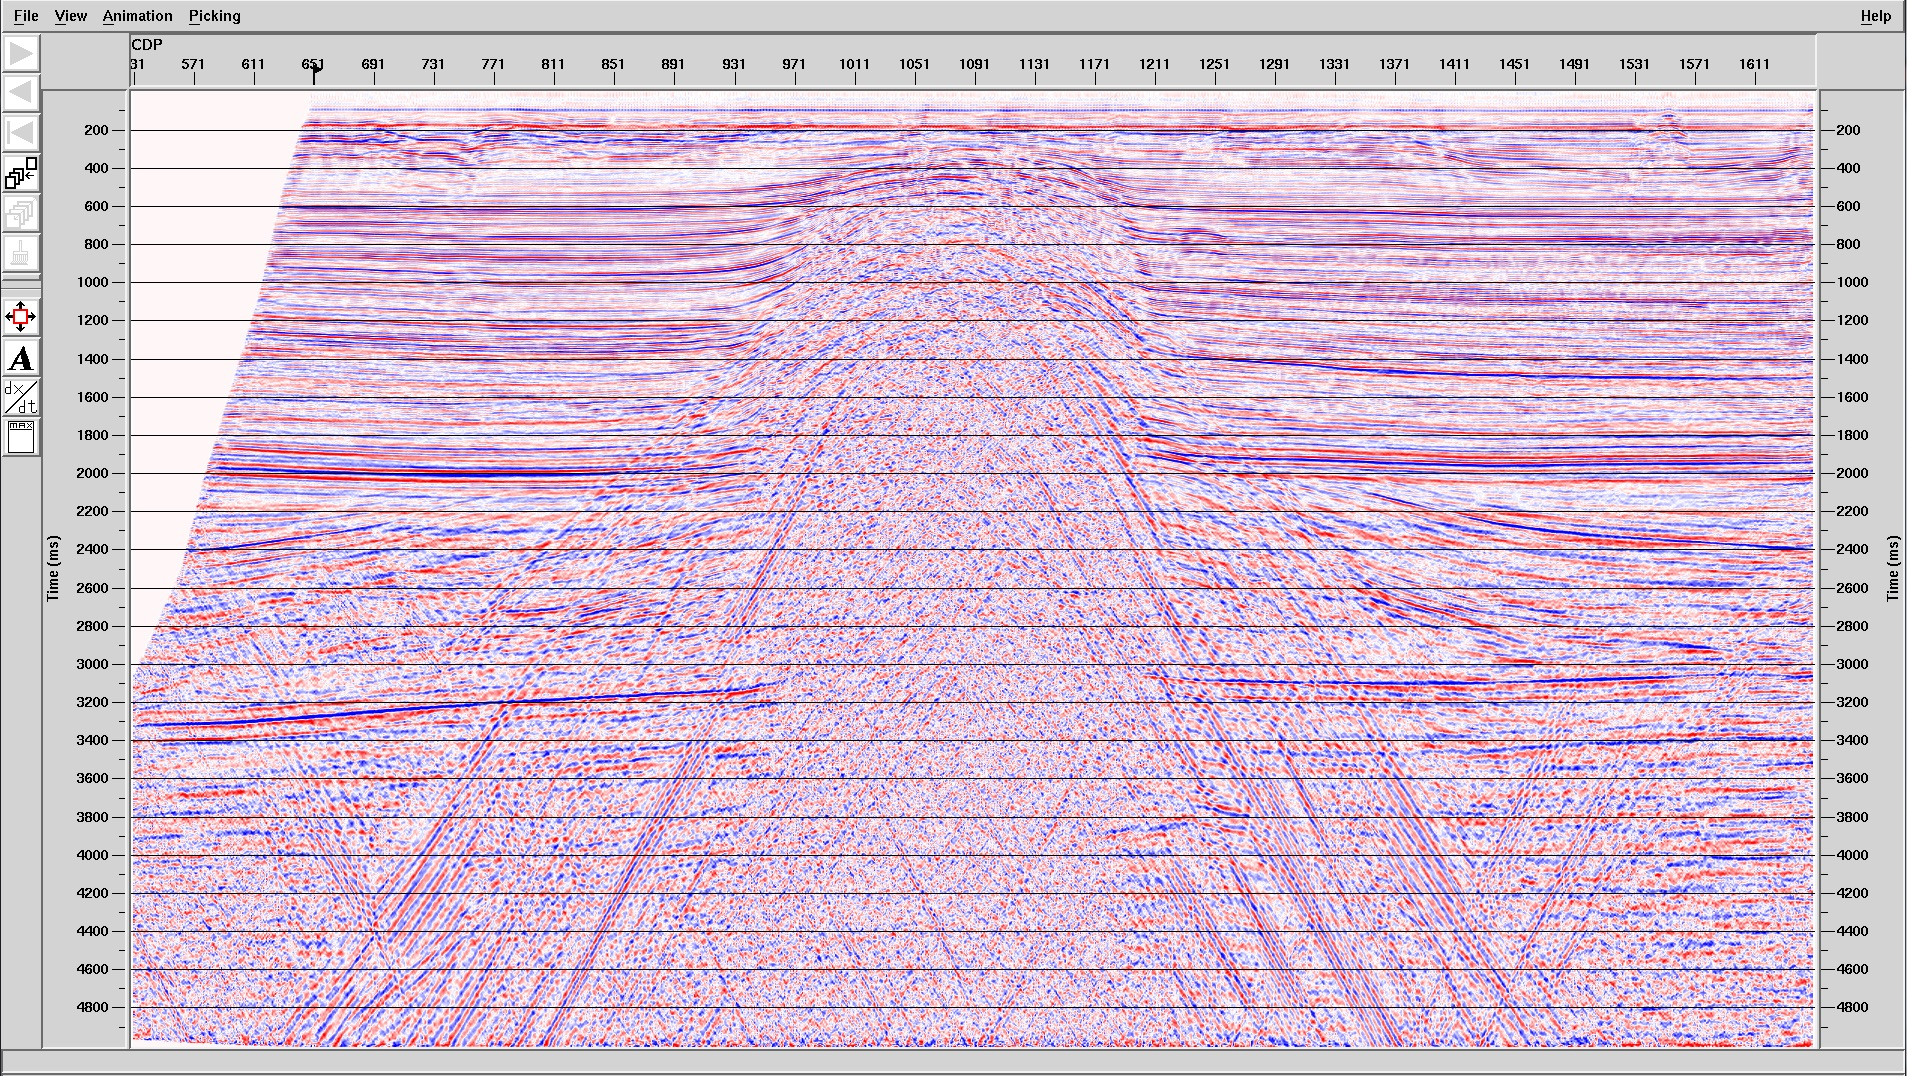
\includegraphics[width=\textwidth]{fmig.jpg}
\caption{Post-stack pre-migration}
\label{fmig}
\end{figure}

\noindent Migration of seismic data aims to relocate seismic features to their true subsurface locations and collapse diffractions, thus increasing spatial resolution and producing a correct seismic image of the subsurface. The procedure of migration consists of two steps:

\begin{itemize}
    \item Downward extrapolation: a simulation involving moving the receivers from the surface down through the model with an arbitrarily small travel time interval
    \item Imaging: for each moved (downward extrapolated) receiver, a new seismic strip is formed. From each strip, only the signals received close to zero offset is kept, to further treat these arriving signals as local secondary sources. Combining these strips forms a migrated section (Gelius, 2018b; Yilmas, 2014)
\end{itemize}

\noindent We separate post-stack and pre-stack migration, along with whether they are performed in time or depth domain. When complexity in velocity is prominent, time migration does not produce a good subsurface image. In such cases depth migration is preferred. In cases with strong complexity in geology, pre-stack is preferred (Gelius, 2018b). See figure \ref{Types}, illustrating the relationship between the different migration processes.

\begin{figure}[H]
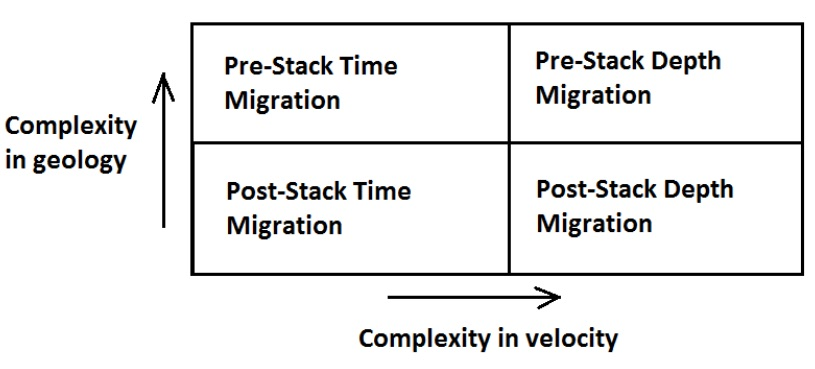
\includegraphics[scale=0.4]{types_of_migration.jpg}
\caption{Illustration showing ideal migration type in relation to complexity in geology and velocity. Modified from Gelius (2018b).}
\label{Types}
\end{figure}

\subsection{Post-Stack Time Migration}

\noindent Post-stack time migration stacks the traces before the events are repositioned to their actual position in time. The disadvantage of post stack time migration is that it only yields good results when the geology and velocity of the model is uncomplicated. Post stack time migrations are usually computationally efficient and should be used when possible. In this project, two types of post stack time migration are used: Finite Difference time migration (FDTM) and Kirchhoff time migration.

\subsection{Finite Difference (FD) Migration}

\noindent FD-migration is based on parabolic approximations of the wave-equation, and can be used to recursively implement downward extrapolations, still handling lateral velocity changes.\\
FD-migration may be implemented in time with dip limitation, by retaining the thin-lense term of the scalar wave equation. FD-migration may also be implemented on steep dips in depth-migration (Gelius, 2018b).
\\
Finite Difference depth-migration (FDDM) can handle significantly large lateral velocity variations, but is highly sensitive to inaccurate migration velocity. Finite Difference time-migration (FDTM) however, can handle only somewhat lateral velocity variations. This requires that the lateral variations are smooth and much smaller than the vertical variations. However, caution is required when performing the migration as FDTM-schemes may cause dispersion effects and contain dip-angle limitations (Gelius, 2018b). 
\\
As the FD-migration is employed in the time domain for this workflow, the $45^{\circ}$ max dip approximation was used. This means that the scheme can handle dips up $45^{\circ}$,. The result of FDTM can be seen in Figure \ref{FDTM}.

\begin{figure}[H]
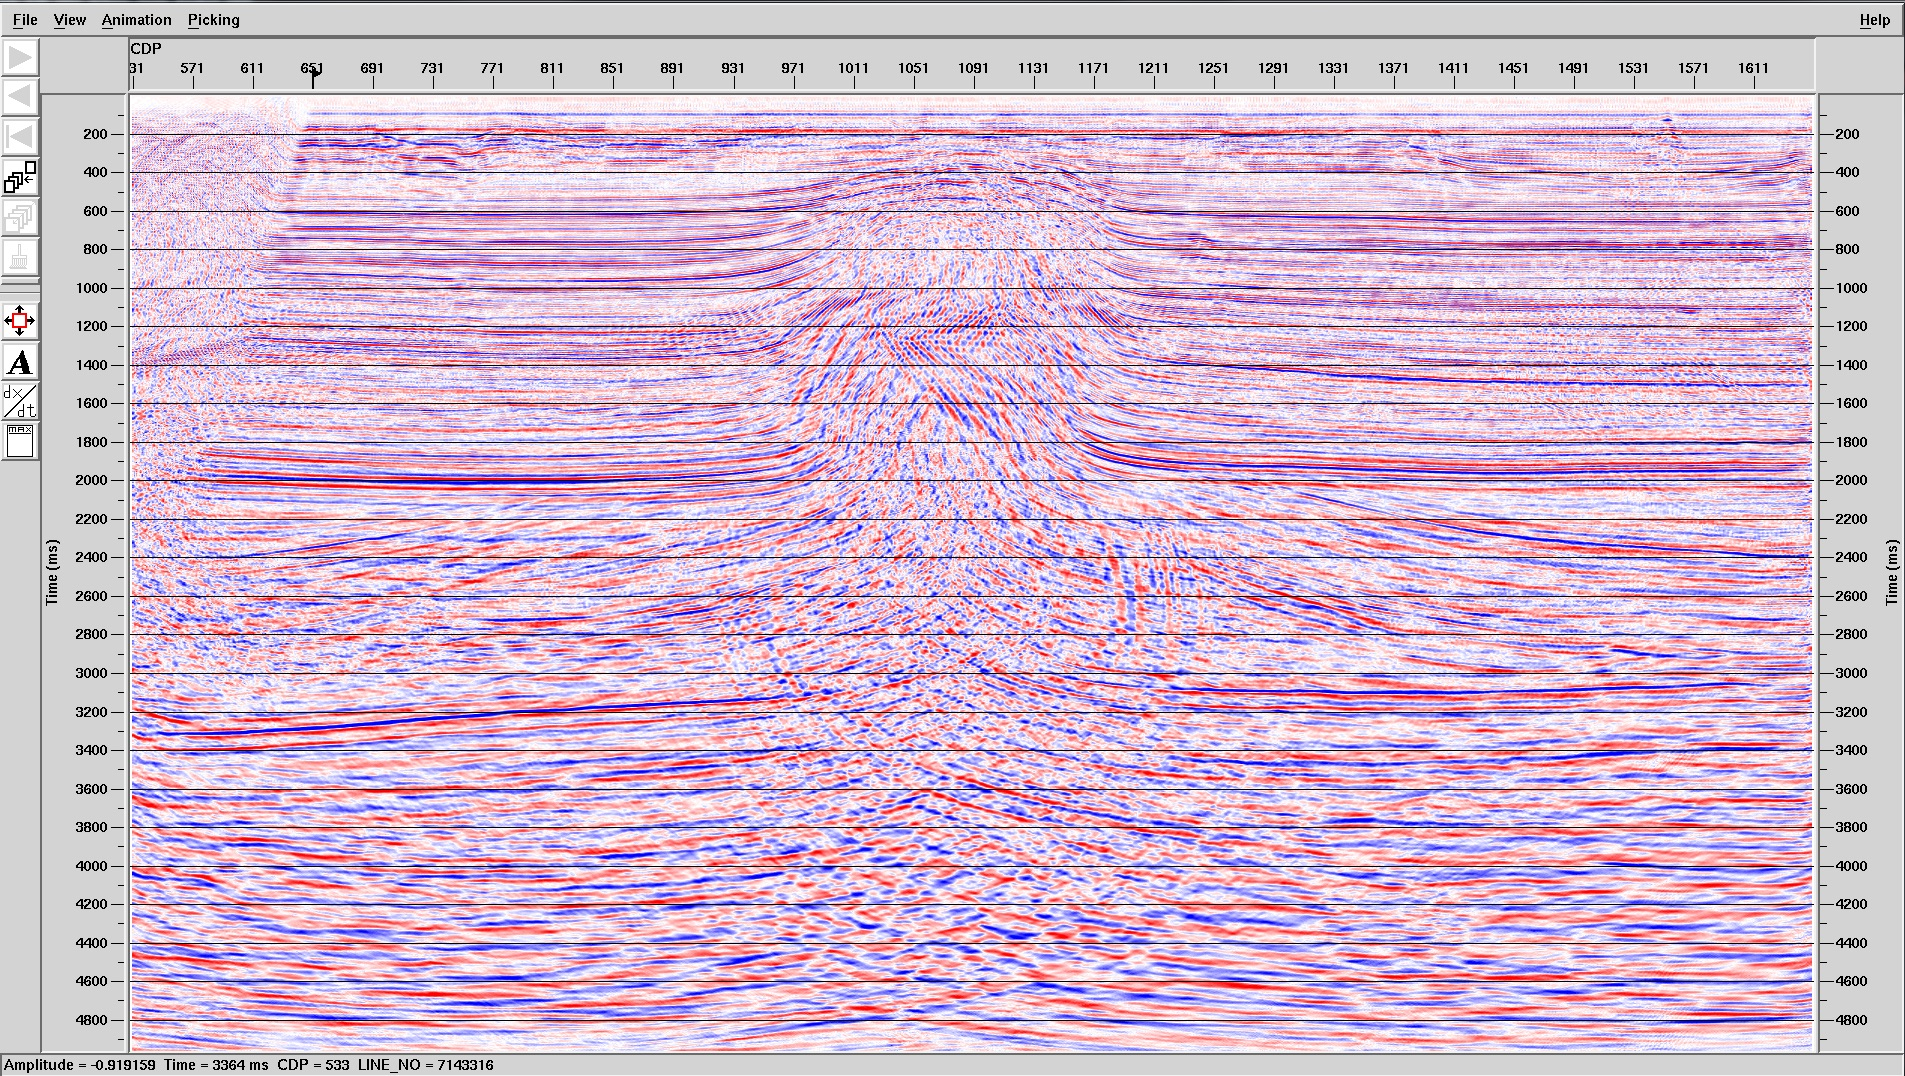
\includegraphics[width=\textwidth]{FDmed3aforkirchh.jpg}
\caption{FDT-migrated section using a $45^{\circ}$ implicit scheme}
\label{FDTM}
\end{figure}

\subsection{Kirchhoff Migration}

The Kirchhoff migration algorithm tries to make a hyperbola that has the best fit with the traces, to then stack all the trace values at the apex of the hyperbola (Figure \ref{KGeoClass}). 

\begin{figure}[H]
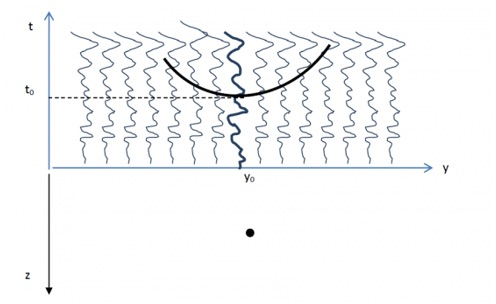
\includegraphics[scale=0.5]{kirchhoffGeoClass.jpg}
\caption{Illustration of how Kirchhoff-migration is stacking traces at the apex of a fitted hyperbola}
\label{KGeoClass}
\end{figure}

\noindent The Kirchhoff migration made in ProMax relies on the velocity function containing the stacking velocities, unlike FD which relies on the migration velocity function which is based on interval velocity. The result of Kirchhoff can be seen on Figure \ref{KTM}.

\begin{figure}[H]
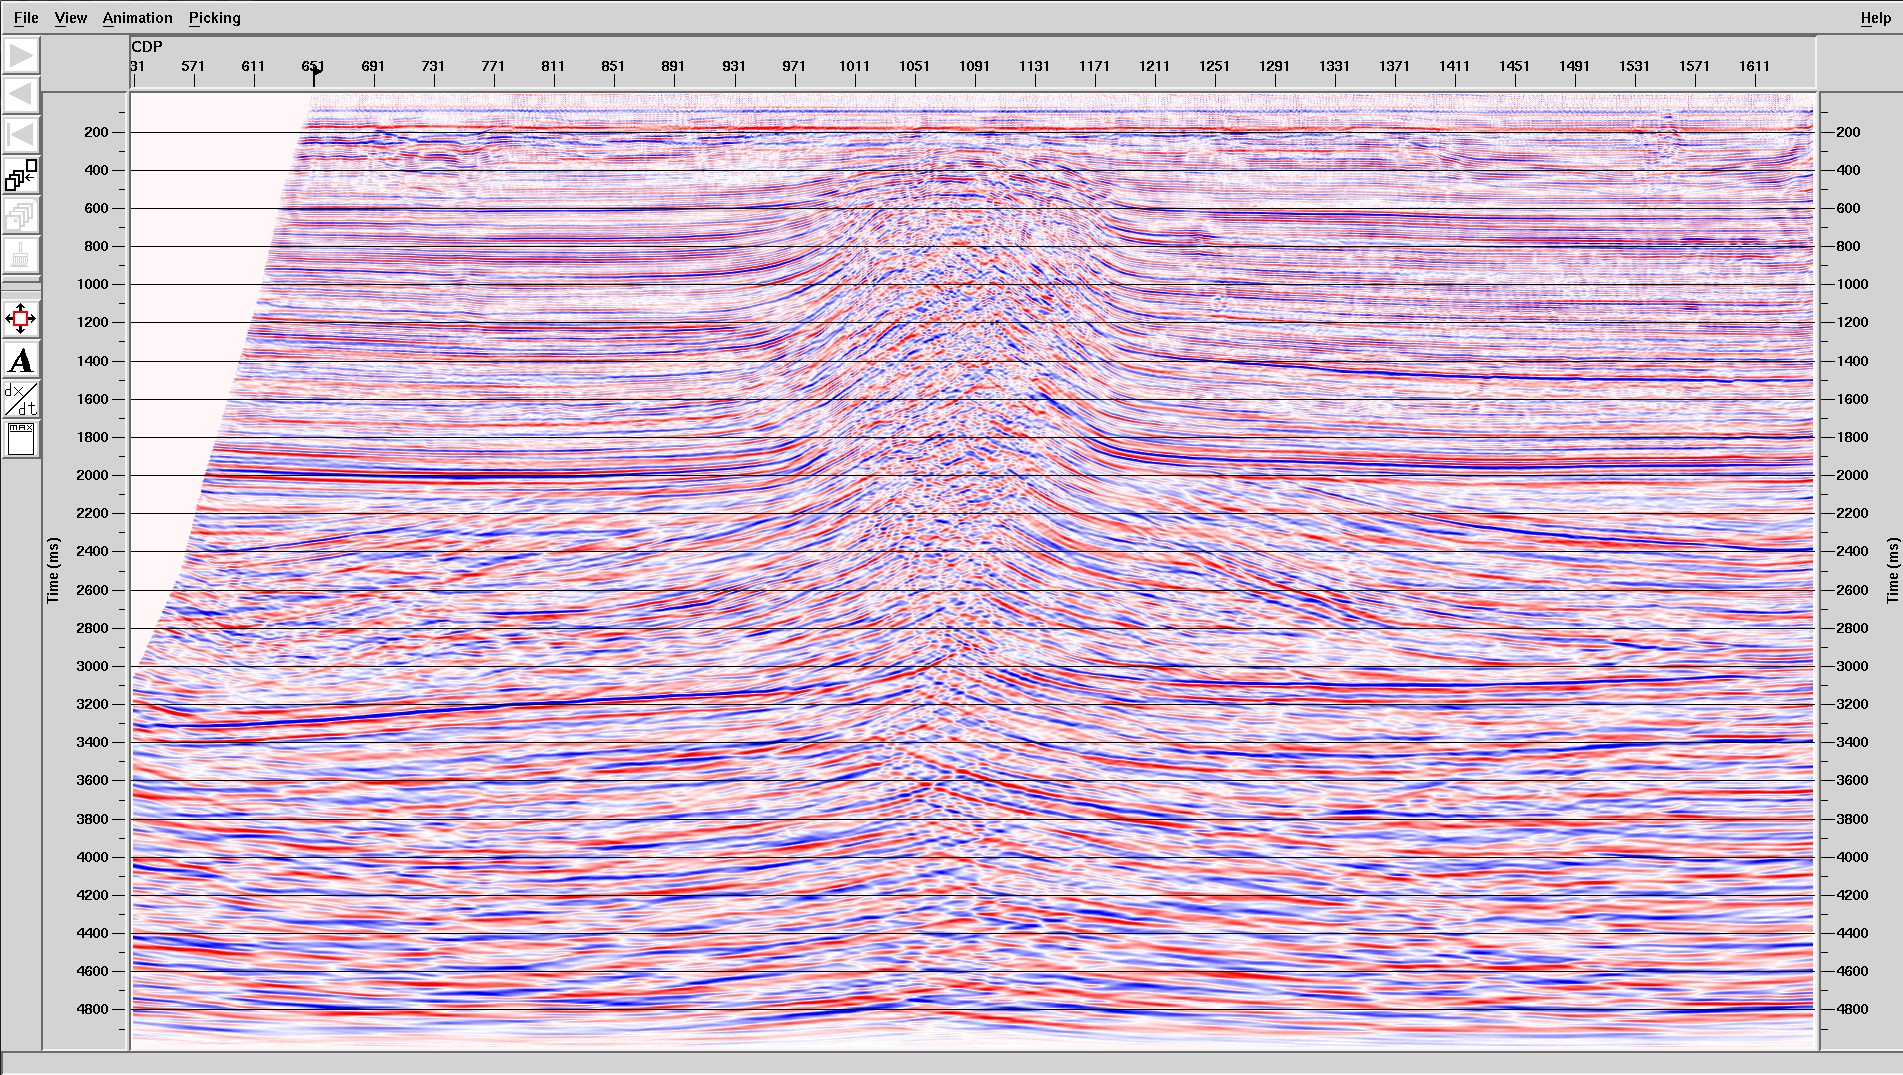
\includegraphics[width=\textwidth]{kirchhmed3aforkirchh.jpg}
\caption{Kirchhoff migrated section}
\label{KTM}
\end{figure}

\section{Observations and comparisons}

The processing done to the dataset during the entire workflow resulted in two migrated sections, one employing FDT-migration, the other employing Kirchhoff-migration. Four main observations were made in comparison of these sections both to each other and to the section prior to migration, see figures \ref{ny1} - \ref{ny3}. 

\begin{figure}[H]
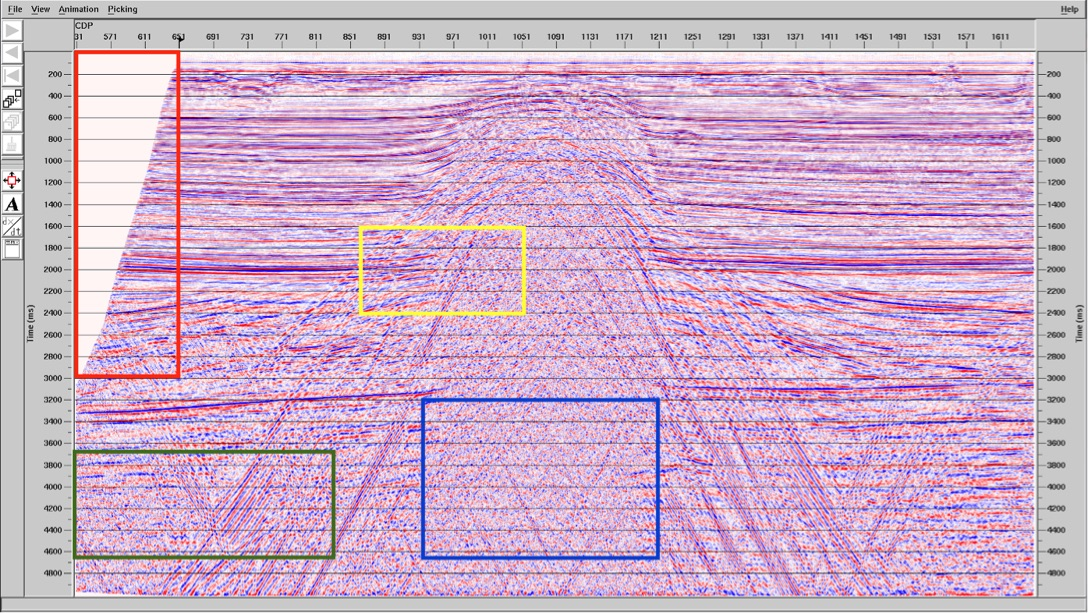
\includegraphics[width=\textwidth]{ny1.jpg}
\caption{Pre-migrated section. Color-coded boxes marks areas of particular interest, which are discussed in detail separately.}
\label{ny1}
\end{figure}

\begin{figure}[H]
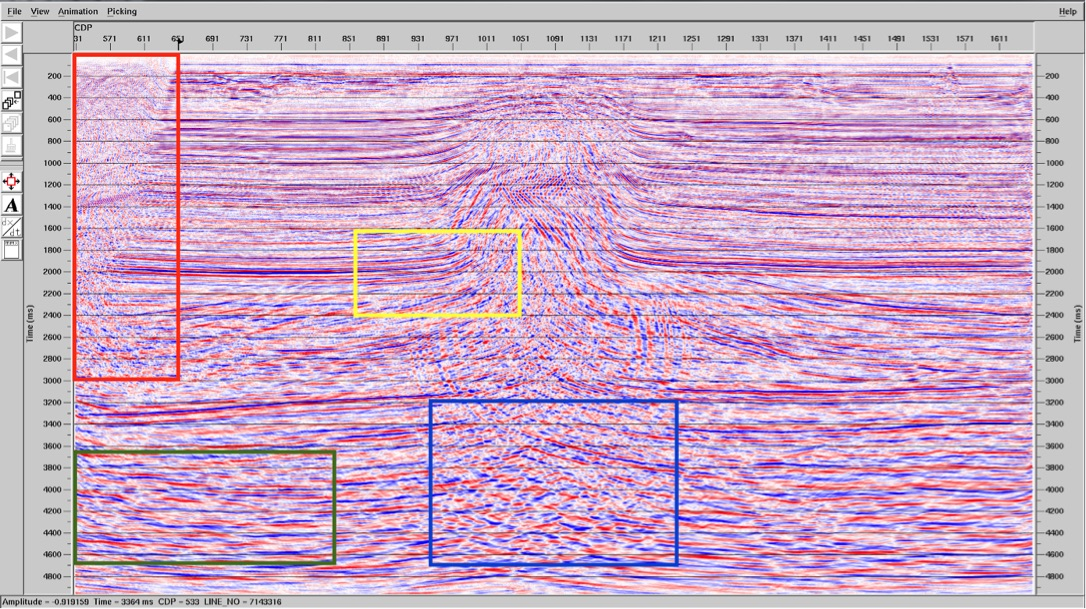
\includegraphics[width=\textwidth]{ny2.jpg}
\caption{FDT-migrated section. Color-coded boxes marks areas of particular interest, which are discussed in detail separately.}
\label{ny2}
\end{figure}

\begin{figure}[H]
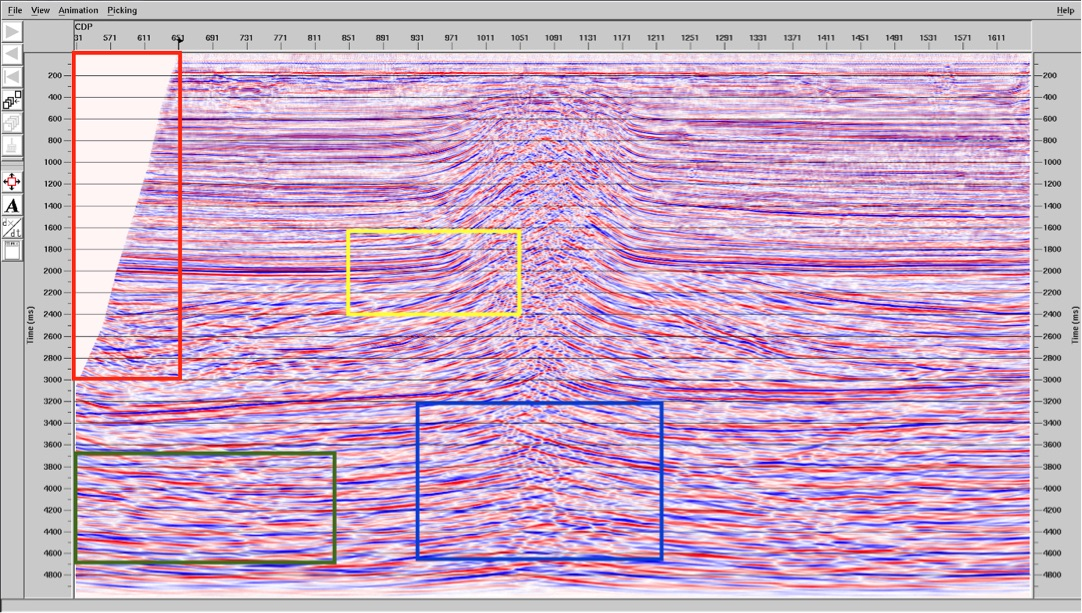
\includegraphics[width=\textwidth]{ny3.jpg}
\caption{Kirchhoff-migrated section. Color-coded boxes marks areas of particular interest, which are discussed in detail separately.}
\label{ny3}
\end{figure}

\subsection{Computed noise and muting}

\begin{figure}[H]
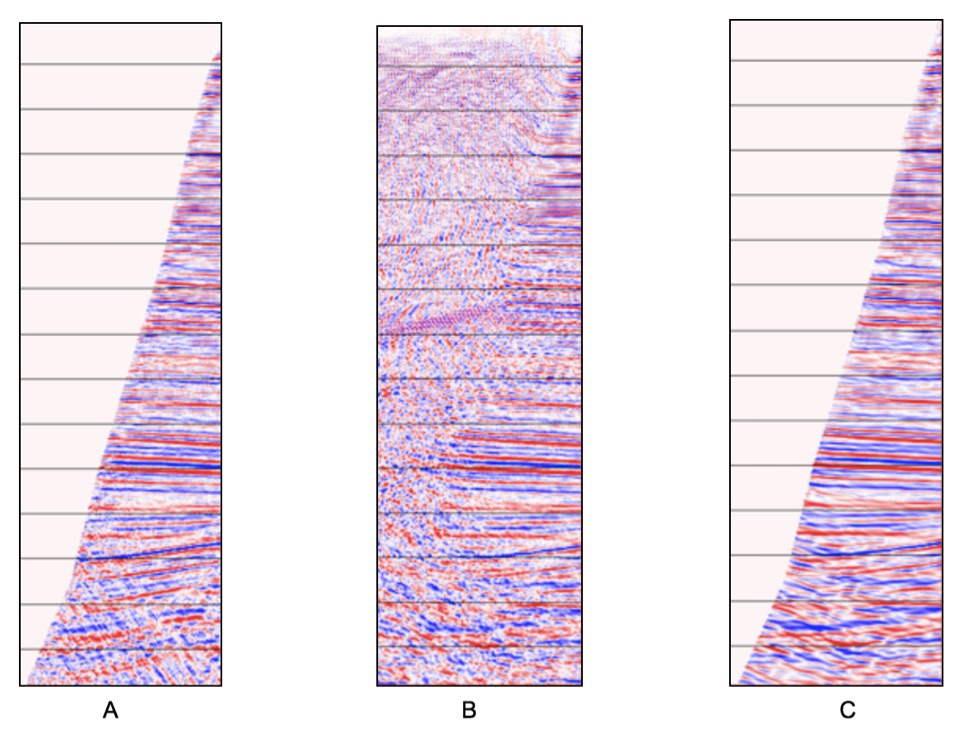
\includegraphics[width=\textwidth]{ny4.jpg}
\caption{Figures show zoomed sections marked in red boxes in figures \ref{ny1} - \ref{ny3}. A: before migration, B: after applying FDT-migration and C: after applying Kirchhoff-migration.}
\label{ny4}
\end{figure}

\noindent Data at low offsets and time is muted and zeroed out with respect to NMO-stretching prior to migration, see figure 39-A. In the FDT-migration, figure 39-B data still appears, despite the mute. This is due to the implicit calculations done using data under the top mute during this type of migration. For the Kirchhoff-migration, figure 39-C however, lack of data at low offsets and time are coincident with the mute-function applied prior to migration. In summary, at these low offsets, Kirchhoff-migration displays a higher S/N-ratio and produces better imaging. 

\subsection{Velocity pull-up}

\begin{figure}[H]
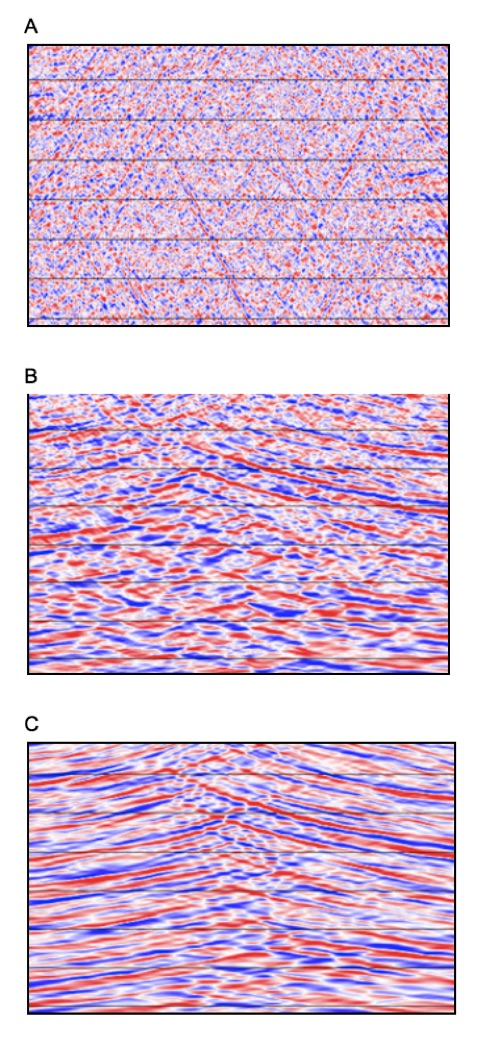
\includegraphics[scale=0.4]{ny5.jpg}
\caption{Figures show zoomed sections marked in blue boxes in figures \ref{ny1} - \ref{ny3}. 
A: before migration, B: after applying FDT-migration and C: after applying Kirchhoff-migration.}
\label{ny5}
\end{figure}

\noindent Figure 40A shows how no reflectors appear below the salt dome and only noise can be observed. Comparing 40A with 40B and 40C shows how both migration types have immense effects on the data. For the FDT-migration, figure 40B, the deeper reflectors become visible under the salt dome. However, these reflectors experience profound velocity pull-up due to the high velocity of salt. To achieve a more accurate depiction of the subsurface, an advanced depth migration has to be implemented, which requires a better velocity model based on depth. For the Kirchhoff-migrated data, figure 40C, beneath the salt, the reflectors are better imaged as they show enhanced evenness and separation. However, the Kirchhoff-migrated data also show signs of velocity pull up, but not to as great an extent as the FDT-migration. 

\subsection{Adjustment of dip}

\begin{figure}[H]
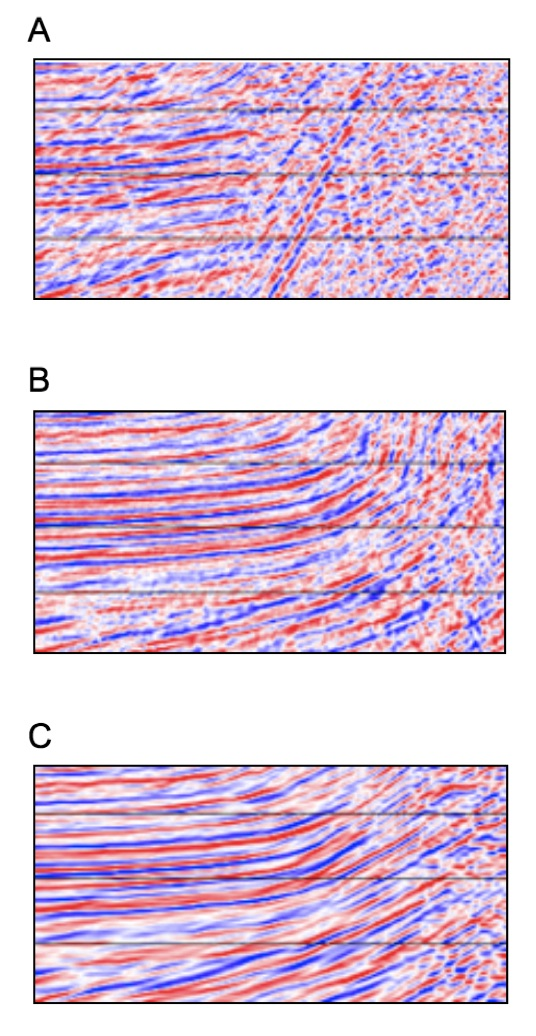
\includegraphics[scale=0.4]{ny6.jpg}
\caption{Figures show zoomed sections marked in yellow boxes in figures \ref{ny1} - \ref{ny3}. A: before migration, B: after applying FDT-migration and C: after applying Kirchhoff-migration. }
\label{ny6}
\end{figure}

Figure 41A-C shows how reflectors at the sides of the salt dome behave with migration. Before migration the reflector appear horizontal, but both FDT- and Kirchhoff-migration show that the reflectors actually dip upwards close to the dome. This is not an effect caused by migration, but rather the true dip of the sedimentary layers. The dip is caused by the salt pushing its way upwards due to buoyancy and in the process tilting the layers. This dip correction shows that both a 45 degree FDTM and Kirchhoff migration are able to handle such steep dips. 

\subsection{Scattering}

\begin{figure}[H]
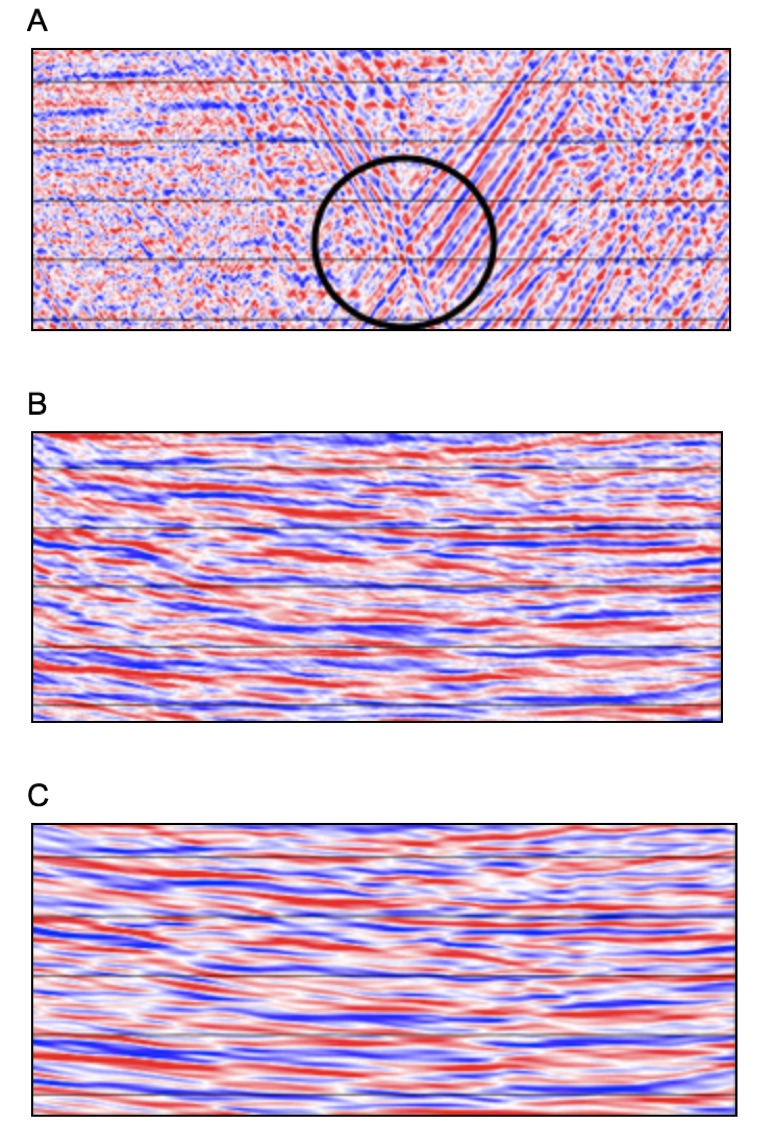
\includegraphics[scale=0.4]{ny7.jpg}
\caption{Figures show zoomed sections marked in green boxes in figures \ref{ny1}-\ref{ny3}. 
A: before migration, B: after applying FDT-migration and C: after applying Kirchhoff-migration. Scattering point circled in black in A.}
\label{ny7}
\end{figure}

\noindent The pre-migrated section (Figure 42-A-C) shows the typical diffraction hyperbola, which is reduced to a scattering point after migration. Both types of migrations seem to handle the collapse of diffraction hyperbolas very well so that true reflectors are revealed. 

\section{Concluding remarks}
The workflow proved highly efficient in processing the data. Although the final results (FDT- and Kirchhoff-migrated sections) contain varying accuracy and S/N-ratios, they both reveal the presence of a salt dome fully enclosed by sedimentary layers. 
\\
Applying a velocity model based on the assumption of small lateral velocity variation somewhat retards the success of both the Kirchhoff- and FDT-migration-schemes. This ought to be taken into consideration for in future studies.
\\
All multiples, not only the seabed multiple could have been removed with intent to increase the accuracy of the NMO-correction. Having the salt dome in mind while doing the velocity analysis would also improve results.
\\
The processes applied in this workflow gave great results, but even more processing could have been done to the data to improve the final image.

\newpage

\section{References}

\begin{itemize}
    \item Baird Petrophysical (2005) Velocity Analysis and NMO-Correction [Online]. Houston: Baird Petrophysical International. Available from: $<http://www.bairdpetro.com/pdf_files/p58-62.pdf>$ [02.05.18]
    \item Gelius, L. J., 2018a. Seismic Signal Theory and Processing, UniGeo: GeoClass 
    \item Gelius, L. J., 2018b. Seismic Imaging, UniGeo: GeoClass
    \item Gillis, G. (2018a) Stack [Online]. Texas: Schlumberger Oilfield Glossary. Available from:\\ $<http://www.glossary.oilfield.slb.com/Terms/s/stack.aspx>$ [30.04.18].
    \item Gillis, G. (2018b) AGC [Online]. Texas: Schlumberger Oilfield Glossary. Available from:\\ $<http://www.glossary.oilfield.slb.com/Terms/a/automatic_gain_control.aspx>$ [30.04.18].
    \item XSGEO (2015) [Online]. Hess Corporation. Available from: $<http://www.xsgeo.com/course/acq.htm>$ [02.05.18]
    \item Yilmaz, O. (2014) Introduction to Migration [Online]. SEG Wiki. Available from:\\ $<http://dx.doi.org/10.1190/1.9781560801580>$ [03.04.18]
\end{itemize}

\end{document}